\documentclass[1p]{elsarticle_modified}
%\bibliographystyle{elsarticle-num}

%\usepackage[colorlinks]{hyperref}
%\usepackage{abbrmath_seonhwa} %\Abb, \Ascr, \Acal ,\Abf, \Afrak
\usepackage{amsfonts}
\usepackage{amssymb}
\usepackage{amsmath}
\usepackage{amsthm}
\usepackage{scalefnt}
\usepackage{amsbsy}
\usepackage{kotex}
\usepackage{caption}
\usepackage{subfig}
\usepackage{color}
\usepackage{graphicx}
\usepackage{xcolor} %% white, black, red, green, blue, cyan, magenta, yellow
\usepackage{float}
\usepackage{setspace}
\usepackage{hyperref}

\usepackage{tikz}
\usetikzlibrary{arrows}

\usepackage{multirow}
\usepackage{array} % fixed length table
\usepackage{hhline}

%%%%%%%%%%%%%%%%%%%%%
\makeatletter
\renewcommand*\env@matrix[1][\arraystretch]{%
	\edef\arraystretch{#1}%
	\hskip -\arraycolsep
	\let\@ifnextchar\new@ifnextchar
	\array{*\c@MaxMatrixCols c}}
\makeatother %https://tex.stackexchange.com/questions/14071/how-can-i-increase-the-line-spacing-in-a-matrix
%%%%%%%%%%%%%%%

\usepackage[normalem]{ulem}

\newcommand{\msout}[1]{\ifmmode\text{\sout{\ensuremath{#1}}}\else\sout{#1}\fi}
%SOURCE: \msout is \stkout macro in https://tex.stackexchange.com/questions/20609/strikeout-in-math-mode

\newcommand{\cancel}[1]{
	\ifmmode
	{\color{red}\msout{#1}}
	\else
	{\color{red}\sout{#1}}
	\fi
}

\newcommand{\add}[1]{
	{\color{blue}\uwave{#1}}
}

\newcommand{\replace}[2]{
	\ifmmode
	{\color{red}\msout{#1}}{\color{blue}\uwave{#2}}
	\else
	{\color{red}\sout{#1}}{\color{blue}\uwave{#2}}
	\fi
}

\newcommand{\Sol}{\mathcal{S}} %segment
\newcommand{\D}{D} %diagram
\newcommand{\A}{\mathcal{A}} %arc


%%%%%%%%%%%%%%%%%%%%%%%%%%%%%5 test

\def\sl{\operatorname{\textup{SL}}(2,\Cbb)}
\def\psl{\operatorname{\textup{PSL}}(2,\Cbb)}
\def\quan{\mkern 1mu \triangleright \mkern 1mu}

\theoremstyle{definition}
\newtheorem{thm}{Theorem}[section]
\newtheorem{prop}[thm]{Proposition}
\newtheorem{lem}[thm]{Lemma}
\newtheorem{ques}[thm]{Question}
\newtheorem{cor}[thm]{Corollary}
\newtheorem{defn}[thm]{Definition}
\newtheorem{exam}[thm]{Example}
\newtheorem{rmk}[thm]{Remark}
\newtheorem{alg}[thm]{Algorithm}

\newcommand{\I}{\sqrt{-1}}
\begin{document}

%\begin{frontmatter}
%
%\title{Boundary parabolic representations of knots up to 8 crossings}
%
%%% Group authors per affiliation:
%\author{Yunhi Cho} 
%\address{Department of Mathematics, University of Seoul, Seoul, Korea}
%\ead{yhcho@uos.ac.kr}
%
%
%\author{Seonhwa Kim} %\fnref{s_kim}}
%\address{Center for Geometry and Physics, Institute for Basic Science, Pohang, 37673, Korea}
%\ead{ryeona17@ibs.re.kr}
%
%\author{Hyuk Kim}
%\address{Department of Mathematical Sciences, Seoul National University, Seoul 08826, Korea}
%\ead{hyukkim@snu.ac.kr}
%
%\author{Seokbeom Yoon}
%\address{Department of Mathematical Sciences, Seoul National University, Seoul, 08826,  Korea}
%\ead{sbyoon15@snu.ac.kr}
%
%\begin{abstract}
%We find all boundary parabolic representation of knots up to 8 crossings.
%
%\end{abstract}
%\begin{keyword}
%    \MSC[2010] 57M25 
%\end{keyword}
%
%\end{frontmatter}

%\linenumbers
%\tableofcontents
%
\newcommand\colored[1]{\textcolor{white}{\rule[-0.35ex]{0.8em}{1.4ex}}\kern-0.8em\color{red} #1}%
%\newcommand\colored[1]{\textcolor{white}{ #1}\kern-2.17ex	\textcolor{white}{ #1}\kern-1.81ex	\textcolor{white}{ #1}\kern-2.15ex\color{red}#1	}

{\Large $\underline{12a_{0780}~(K12a_{0780})}$}

\setlength{\tabcolsep}{10pt}
\renewcommand{\arraystretch}{1.6}
\vspace{1cm}\begin{tabular}{m{100pt}>{\centering\arraybackslash}m{274pt}}
\multirow{5}{120pt}{
	\centering
	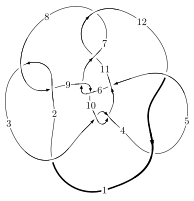
\includegraphics[width=112pt]{../../../GIT/diagram.site/Diagrams/png/1581_12a_0780.png}\\
\ \ \ A knot diagram\footnotemark}&
\allowdisplaybreaks
\textbf{Linearized knot diagam} \\
\cline{2-2}
 &
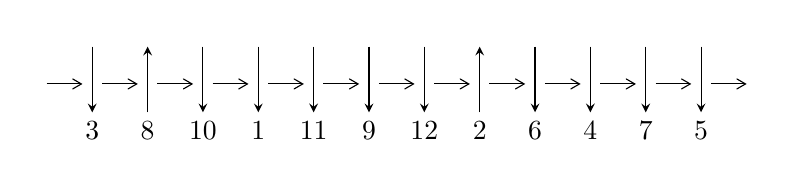
\begin{tikzpicture}[x=20pt, y=17pt]
	% nodes
	\node (C0) at (0, 0) {};
	\node (C1) at (1, 0) {};
	\node (C1U) at (1, +1) {};
	\node (C1D) at (1, -1) {3};

	\node (C2) at (2, 0) {};
	\node (C2U) at (2, +1) {};
	\node (C2D) at (2, -1) {8};

	\node (C3) at (3, 0) {};
	\node (C3U) at (3, +1) {};
	\node (C3D) at (3, -1) {10};

	\node (C4) at (4, 0) {};
	\node (C4U) at (4, +1) {};
	\node (C4D) at (4, -1) {1};

	\node (C5) at (5, 0) {};
	\node (C5U) at (5, +1) {};
	\node (C5D) at (5, -1) {11};

	\node (C6) at (6, 0) {};
	\node (C6U) at (6, +1) {};
	\node (C6D) at (6, -1) {9};

	\node (C7) at (7, 0) {};
	\node (C7U) at (7, +1) {};
	\node (C7D) at (7, -1) {12};

	\node (C8) at (8, 0) {};
	\node (C8U) at (8, +1) {};
	\node (C8D) at (8, -1) {2};

	\node (C9) at (9, 0) {};
	\node (C9U) at (9, +1) {};
	\node (C9D) at (9, -1) {6};

	\node (C10) at (10, 0) {};
	\node (C10U) at (10, +1) {};
	\node (C10D) at (10, -1) {4};

	\node (C11) at (11, 0) {};
	\node (C11U) at (11, +1) {};
	\node (C11D) at (11, -1) {7};

	\node (C12) at (12, 0) {};
	\node (C12U) at (12, +1) {};
	\node (C12D) at (12, -1) {5};
	\node (C13) at (13, 0) {};

	% arrows
	\draw[->,>={angle 60}]
	(C0) edge (C1) (C1) edge (C2) (C2) edge (C3) (C3) edge (C4) (C4) edge (C5) (C5) edge (C6) (C6) edge (C7) (C7) edge (C8) (C8) edge (C9) (C9) edge (C10) (C10) edge (C11) (C11) edge (C12) (C12) edge (C13) ;	\draw[->,>=stealth]
	(C1U) edge (C1D) (C2D) edge (C2U) (C3U) edge (C3D) (C4U) edge (C4D) (C5U) edge (C5D) (C6U) edge (C6D) (C7U) edge (C7D) (C8D) edge (C8U) (C9U) edge (C9D) (C10U) edge (C10D) (C11U) edge (C11D) (C12U) edge (C12D) ;
	\end{tikzpicture} \\
\hhline{~~} \\& 
\textbf{Solving Sequence} \\ \cline{2-2} 
 &
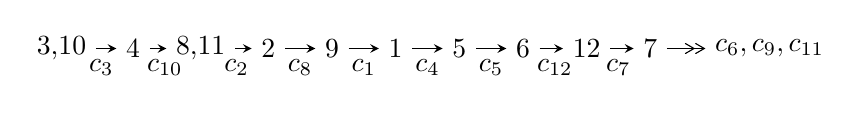
\begin{tikzpicture}[x=23pt, y=7pt]
	% node
	\node (A0) at (-1/8, 0) {3,10};
	\node (A1) at (1, 0) {4};
	\node (A2) at (33/16, 0) {8,11};
	\node (A3) at (25/8, 0) {2};
	\node (A4) at (33/8, 0) {9};
	\node (A5) at (41/8, 0) {1};
	\node (A6) at (49/8, 0) {5};
	\node (A7) at (57/8, 0) {6};
	\node (A8) at (65/8, 0) {12};
	\node (A9) at (73/8, 0) {7};
	\node (C1) at (1/2, -1) {$c_{3}$};
	\node (C2) at (3/2, -1) {$c_{10}$};
	\node (C3) at (21/8, -1) {$c_{2}$};
	\node (C4) at (29/8, -1) {$c_{8}$};
	\node (C5) at (37/8, -1) {$c_{1}$};
	\node (C6) at (45/8, -1) {$c_{4}$};
	\node (C7) at (53/8, -1) {$c_{5}$};
	\node (C8) at (61/8, -1) {$c_{12}$};
	\node (C9) at (69/8, -1) {$c_{7}$};
	\node (A10) at (11, 0) {$c_{6},c_{9},c_{11}$};

	% edge
	\draw[->,>=stealth]	
	(A0) edge (A1) (A1) edge (A2) (A2) edge (A3) (A3) edge (A4) (A4) edge (A5) (A5) edge (A6) (A6) edge (A7) (A7) edge (A8) (A8) edge (A9) ;
	\draw[->>,>={angle 60}]	
	(A9) edge (A10);
\end{tikzpicture} \\ 

\end{tabular} \\

\footnotetext{
The image of knot diagram is generated by the software ``\textbf{Draw programme}" developed by Andrew Bartholomew(\url{http://www.layer8.co.uk/maths/draw/index.htm\#Running-draw}), where we modified some parts for our purpose(\url{https://github.com/CATsTAILs/LinksPainter}).
}\phantom \\ \newline 
\centering \textbf{Ideals for irreducible components\footnotemark of $X_{\text{par}}$} 
 
\begin{align*}
I^u_{1}&=\langle 
-2.19508\times10^{19} u^{30}+3.73360\times10^{19} u^{29}+\cdots+4.83245\times10^{19} b+3.36053\times10^{19},\\
\phantom{I^u_{1}}&\phantom{= \langle  }2.65488\times10^{19} u^{30}-4.25989\times10^{19} u^{29}+\cdots+4.83245\times10^{19} a-9.79800\times10^{19},\;u^{31}- u^{30}+\cdots+4 u^2-1\rangle \\
I^u_{2}&=\langle 
6.81132\times10^{282} u^{103}+3.29331\times10^{282} u^{102}+\cdots+2.47281\times10^{283} b+2.22084\times10^{285},\\
\phantom{I^u_{2}}&\phantom{= \langle  }4.11438\times10^{284} u^{103}+2.15076\times10^{284} u^{102}+\cdots+1.47544\times10^{285} a+1.58373\times10^{287},\\
\phantom{I^u_{2}}&\phantom{= \langle  }u^{104}+u^{103}+\cdots+1113 u+179\rangle \\
I^u_{3}&=\langle 
2.88283\times10^{16} u^{39}+2.47312\times10^{16} u^{38}+\cdots+5.40032\times10^{14} b-1.88417\times10^{16},\\
\phantom{I^u_{3}}&\phantom{= \langle  }5041365482875379 u^{39}-1853997132134618 u^{38}+\cdots+49093794862181 a+5201527324398439,\\
\phantom{I^u_{3}}&\phantom{= \langle  }u^{40}-13 u^{38}+\cdots+u+1\rangle \\
I^u_{4}&=\langle 
- u^5- u^3+u^2+b+u,\;u^7- u^6+2 u^5-3 u^4- u^2+a- u+2,\;u^8+u^6- u^5-2 u^4+u+1\rangle \\
I^u_{5}&=\langle 
402075 u^{23}+134432 u^{22}+\cdots+844628 b-3815144,\\
\phantom{I^u_{5}}&\phantom{= \langle  }1297281615 u^{23}+828936233 u^{22}+\cdots+956118896 a-5354919116,\;u^{24}-4 u^{22}+\cdots-14 u+4\rangle \\
I^u_{6}&=\langle 
b,\;a+1,\;u+1\rangle \\
\\
\end{align*}
\raggedright * 6 irreducible components of $\dim_{\mathbb{C}}=0$, with total 208 representations.\\
\footnotetext{All coefficients of polynomials are rational numbers. But the coefficients are sometimes approximated in decimal forms when there is not enough margin.}
\newpage
\renewcommand{\arraystretch}{1}
\centering \section*{I. $I^u_{1}= \langle -2.20\times10^{19} u^{30}+3.73\times10^{19} u^{29}+\cdots+4.83\times10^{19} b+3.36\times10^{19},\;2.65\times10^{19} u^{30}-4.26\times10^{19} u^{29}+\cdots+4.83\times10^{19} a-9.80\times10^{19},\;u^{31}- u^{30}+\cdots+4 u^2-1 \rangle$}
\flushleft \textbf{(i) Arc colorings}\\
\begin{tabular}{m{7pt} m{180pt} m{7pt} m{180pt} }
\flushright $a_{3}=$&$\begin{pmatrix}1\\0\end{pmatrix}$ \\
\flushright $a_{10}=$&$\begin{pmatrix}0\\u\end{pmatrix}$ \\
\flushright $a_{4}=$&$\begin{pmatrix}1\\u^2\end{pmatrix}$ \\
\flushright $a_{8}=$&$\begin{pmatrix}-0.549385 u^{30}+0.881518 u^{29}+\cdots-1.41104 u+2.02754\\0.454238 u^{30}-0.772609 u^{29}+\cdots+0.861654 u-0.695408\end{pmatrix}$ \\
\flushright $a_{11}=$&$\begin{pmatrix}- u\\- u^3+u\end{pmatrix}$ \\
\flushright $a_{2}=$&$\begin{pmatrix}-0.222511 u^{30}+0.978508 u^{29}+\cdots-2.10042 u+2.65064\\0.713966 u^{30}-1.10192 u^{29}+\cdots+2.28533 u-1.27168\end{pmatrix}$ \\
\flushright $a_{9}=$&$\begin{pmatrix}0.400492 u^{30}-0.295551 u^{29}+\cdots-3.68422 u+2.01348\\0.987830 u^{30}-1.78027 u^{29}+\cdots+6.06348 u-2.16930\end{pmatrix}$ \\
\flushright $a_{1}=$&$\begin{pmatrix}0.491456 u^{30}-0.123412 u^{29}+\cdots+0.184905 u+1.37896\\0.713966 u^{30}-1.10192 u^{29}+\cdots+2.28533 u-1.27168\end{pmatrix}$ \\
\flushright $a_{5}=$&$\begin{pmatrix}2.35112 u^{30}-2.14216 u^{29}+\cdots+6.17496 u-0.993465\\0.995518 u^{30}-0.205887 u^{29}+\cdots+4.36460 u+0.609450\end{pmatrix}$ \\
\flushright $a_{6}=$&$\begin{pmatrix}1.63972 u^{30}-1.94514 u^{29}+\cdots+3.71889 u-1.79387\\1.69270 u^{30}-0.224587 u^{29}+\cdots+6.10926 u+0.895478\end{pmatrix}$ \\
\flushright $a_{12}=$&$\begin{pmatrix}0.0447065 u^{30}+0.378481 u^{29}+\cdots+3.07225 u-0.126197\\-0.332133 u^{30}+0.427280 u^{29}+\cdots-2.02754 u+0.549385\end{pmatrix}$ \\
\flushright $a_{7}=$&$\begin{pmatrix}-0.126197 u^{30}+0.170904 u^{29}+\cdots-1.53724 u+2.07225\\0.549385 u^{30}-0.881518 u^{29}+\cdots+1.41104 u-1.02754\end{pmatrix}$\\&\end{tabular}
\flushleft \textbf{(ii) Obstruction class $= -1$}\\~\\
\flushleft \textbf{(iii) Cusp Shapes $= -\frac{10502766013328767806}{4832454620042859899} u^{30}+\frac{9053641948115436650}{4832454620042859899} u^{29}+\cdots-\frac{13369065530498617863}{4832454620042859899} u-\frac{55516682932002117692}{4832454620042859899}$}\\~\\
\newpage\renewcommand{\arraystretch}{1}
\flushleft \textbf{(iv) u-Polynomials at the component}\newline \\
\begin{tabular}{m{50pt}|m{274pt}}
Crossings & \hspace{64pt}u-Polynomials at each crossing \\
\hline $$\begin{aligned}c_{1}\end{aligned}$$&$\begin{aligned}
&u^{31}+13 u^{30}+\cdots-5076 u-1296
\end{aligned}$\\
\hline $$\begin{aligned}c_{2},c_{8}\end{aligned}$$&$\begin{aligned}
&u^{31}- u^{30}+\cdots-54 u+36
\end{aligned}$\\
\hline $$\begin{aligned}c_{3},c_{7},c_{10}\\c_{11}\end{aligned}$$&$\begin{aligned}
&u^{31}+u^{30}+\cdots-4 u^2+1
\end{aligned}$\\
\hline $$\begin{aligned}c_{4},c_{6},c_{9}\\c_{12}\end{aligned}$$&$\begin{aligned}
&u^{31}-2 u^{30}+\cdots+3 u+1
\end{aligned}$\\
\hline $$\begin{aligned}c_{5}\end{aligned}$$&$\begin{aligned}
&u^{31}+6 u^{30}+\cdots+6656 u+1024
\end{aligned}$\\
\hline
\end{tabular}\\~\\
\newpage\renewcommand{\arraystretch}{1}
\flushleft \textbf{(v) Riley Polynomials at the component}\newline \\
\begin{tabular}{m{50pt}|m{274pt}}
Crossings & \hspace{64pt}Riley Polynomials at each crossing \\
\hline $$\begin{aligned}c_{1}\end{aligned}$$&$\begin{aligned}
&y^{31}+13 y^{30}+\cdots+17064432 y-1679616
\end{aligned}$\\
\hline $$\begin{aligned}c_{2},c_{8}\end{aligned}$$&$\begin{aligned}
&y^{31}+13 y^{30}+\cdots-5076 y-1296
\end{aligned}$\\
\hline $$\begin{aligned}c_{3},c_{7},c_{10}\\c_{11}\end{aligned}$$&$\begin{aligned}
&y^{31}-11 y^{30}+\cdots+8 y-1
\end{aligned}$\\
\hline $$\begin{aligned}c_{4},c_{6},c_{9}\\c_{12}\end{aligned}$$&$\begin{aligned}
&y^{31}+18 y^{30}+\cdots+13 y-1
\end{aligned}$\\
\hline $$\begin{aligned}c_{5}\end{aligned}$$&$\begin{aligned}
&y^{31}+2 y^{30}+\cdots-1310720 y-1048576
\end{aligned}$\\
\hline
\end{tabular}\\~\\
\newpage\flushleft \textbf{(vi) Complex Volumes and Cusp Shapes}
$$\begin{array}{c|c|c}  
\text{Solutions to }I^u_{1}& \I (\text{vol} + \sqrt{-1}CS) & \text{Cusp shape}\\
 \hline 
\begin{aligned}
u &= -0.904739 + 0.291878 I \\
a &= \phantom{-}0.65346 - 1.50562 I \\
b &= -0.702786 + 0.584481 I\end{aligned}
 & -3.78119 + 0.29851 I & -10.04466 - 5.69317 I \\ \hline\begin{aligned}
u &= -0.904739 - 0.291878 I \\
a &= \phantom{-}0.65346 + 1.50562 I \\
b &= -0.702786 - 0.584481 I\end{aligned}
 & -3.78119 - 0.29851 I & -10.04466 + 5.69317 I \\ \hline\begin{aligned}
u &= -1.023540 + 0.276276 I \\
a &= -1.127830 + 0.645457 I \\
b &= \phantom{-}0.426119 + 1.184880 I\end{aligned}
 & -4.48013 + 3.96005 I & -9.16910 - 4.26747 I \\ \hline\begin{aligned}
u &= -1.023540 - 0.276276 I \\
a &= -1.127830 - 0.645457 I \\
b &= \phantom{-}0.426119 - 1.184880 I\end{aligned}
 & -4.48013 - 3.96005 I & -9.16910 + 4.26747 I \\ \hline\begin{aligned}
u &= \phantom{-}1.005490 + 0.429232 I \\
a &= \phantom{-}2.30114 + 0.46275 I \\
b &= -0.624836 + 1.042950 I\end{aligned}
 & -5.18236 - 5.45253 I & -10.41007 + 8.28014 I \\ \hline\begin{aligned}
u &= \phantom{-}1.005490 - 0.429232 I \\
a &= \phantom{-}2.30114 - 0.46275 I \\
b &= -0.624836 - 1.042950 I\end{aligned}
 & -5.18236 + 5.45253 I & -10.41007 - 8.28014 I \\ \hline\begin{aligned}
u &= \phantom{-}1.059200 + 0.322674 I \\
a &= -0.92727 - 1.08013 I \\
b &= \phantom{-}0.70406 - 1.33659 I\end{aligned}
 & \phantom{-}1.36245 - 7.78965 I & -7.00543 + 8.80272 I \\ \hline\begin{aligned}
u &= \phantom{-}1.059200 - 0.322674 I \\
a &= -0.92727 + 1.08013 I \\
b &= \phantom{-}0.70406 + 1.33659 I\end{aligned}
 & \phantom{-}1.36245 + 7.78965 I & -7.00543 - 8.80272 I \\ \hline\begin{aligned}
u &= \phantom{-}0.796557 + 0.316743 I \\
a &= -1.160500 - 0.402760 I \\
b &= \phantom{-}1.20965 - 0.90259 I\end{aligned}
 & \phantom{-}5.08416 - 5.15512 I & -3.79747 + 9.54392 I \\ \hline\begin{aligned}
u &= \phantom{-}0.796557 - 0.316743 I \\
a &= -1.160500 + 0.402760 I \\
b &= \phantom{-}1.20965 + 0.90259 I\end{aligned}
 & \phantom{-}5.08416 + 5.15512 I & -3.79747 - 9.54392 I\\
 \hline 
 \end{array}$$\newpage$$\begin{array}{c|c|c}  
\text{Solutions to }I^u_{1}& \I (\text{vol} + \sqrt{-1}CS) & \text{Cusp shape}\\
 \hline 
\begin{aligned}
u &= -0.667071 + 0.461492 I \\
a &= \phantom{-}0.280234 + 0.536083 I \\
b &= \phantom{-}0.882837 + 0.031450 I\end{aligned}
 & \phantom{-}5.33055 + 1.69004 I & -1.97215 - 4.21413 I \\ \hline\begin{aligned}
u &= -0.667071 - 0.461492 I \\
a &= \phantom{-}0.280234 - 0.536083 I \\
b &= \phantom{-}0.882837 - 0.031450 I\end{aligned}
 & \phantom{-}5.33055 - 1.69004 I & -1.97215 + 4.21413 I \\ \hline\begin{aligned}
u &= \phantom{-}1.195060 + 0.171054 I \\
a &= -0.520257 - 1.094170 I \\
b &= -0.159112 - 1.058030 I\end{aligned}
 & -8.22893 + 0.97469 I & -16.7057 - 1.4101 I \\ \hline\begin{aligned}
u &= \phantom{-}1.195060 - 0.171054 I \\
a &= -0.520257 + 1.094170 I \\
b &= -0.159112 + 1.058030 I\end{aligned}
 & -8.22893 - 0.97469 I & -16.7057 + 1.4101 I \\ \hline\begin{aligned}
u &= \phantom{-}0.740357\phantom{ +0.000000I} \\
a &= -0.402635\phantom{ +0.000000I} \\
b &= \phantom{-}0.633812\phantom{ +0.000000I}\end{aligned}
 & -1.21453\phantom{ +0.000000I} & -8.10490\phantom{ +0.000000I} \\ \hline\begin{aligned}
u &= -1.188210 + 0.435471 I \\
a &= -0.401213 + 0.319230 I \\
b &= \phantom{-}0.01900 + 1.52100 I\end{aligned}
 & -4.40480 + 9.52849 I & -10.46510 - 9.09050 I \\ \hline\begin{aligned}
u &= -1.188210 - 0.435471 I \\
a &= -0.401213 - 0.319230 I \\
b &= \phantom{-}0.01900 - 1.52100 I\end{aligned}
 & -4.40480 - 9.52849 I & -10.46510 + 9.09050 I \\ \hline\begin{aligned}
u &= -0.666570 + 1.157020 I \\
a &= \phantom{-}1.379760 - 0.003498 I \\
b &= -0.724812 - 0.579148 I\end{aligned}
 & \phantom{-}7.48792 - 0.22792 I & -1.69345 + 0.87575 I \\ \hline\begin{aligned}
u &= -0.666570 - 1.157020 I \\
a &= \phantom{-}1.379760 + 0.003498 I \\
b &= -0.724812 + 0.579148 I\end{aligned}
 & \phantom{-}7.48792 + 0.22792 I & -1.69345 - 0.87575 I \\ \hline\begin{aligned}
u &= \phantom{-}0.268926 + 1.349580 I \\
a &= \phantom{-}1.164290 - 0.318035 I \\
b &= -0.220775 + 0.993543 I\end{aligned}
 & \phantom{-}3.13273 - 0.69529 I & -3.01718 - 5.31456 I\\
 \hline 
 \end{array}$$\newpage$$\begin{array}{c|c|c}  
\text{Solutions to }I^u_{1}& \I (\text{vol} + \sqrt{-1}CS) & \text{Cusp shape}\\
 \hline 
\begin{aligned}
u &= \phantom{-}0.268926 - 1.349580 I \\
a &= \phantom{-}1.164290 + 0.318035 I \\
b &= -0.220775 - 0.993543 I\end{aligned}
 & \phantom{-}3.13273 + 0.69529 I & -3.01718 + 5.31456 I \\ \hline\begin{aligned}
u &= \phantom{-}1.202140 + 0.675507 I \\
a &= \phantom{-}0.715667 + 0.660411 I \\
b &= -1.069400 - 0.469167 I\end{aligned}
 & \phantom{-}3.20086 - 13.35560 I & -6.05212 + 7.56492 I \\ \hline\begin{aligned}
u &= \phantom{-}1.202140 - 0.675507 I \\
a &= \phantom{-}0.715667 - 0.660411 I \\
b &= -1.069400 + 0.469167 I\end{aligned}
 & \phantom{-}3.20086 + 13.35560 I & -6.05212 - 7.56492 I \\ \hline\begin{aligned}
u &= \phantom{-}0.63713 + 1.30118 I \\
a &= \phantom{-}0.964989 + 0.428697 I \\
b &= -0.630715 - 1.038540 I\end{aligned}
 & \phantom{-}6.10362 + 5.43386 I & -5.40395 - 7.12702 I \\ \hline\begin{aligned}
u &= \phantom{-}0.63713 - 1.30118 I \\
a &= \phantom{-}0.964989 - 0.428697 I \\
b &= -0.630715 + 1.038540 I\end{aligned}
 & \phantom{-}6.10362 - 5.43386 I & -5.40395 + 7.12702 I \\ \hline\begin{aligned}
u &= -1.28784 + 0.72177 I \\
a &= \phantom{-}1.60965 - 0.43290 I \\
b &= -0.720905 - 1.192920 I\end{aligned}
 & \phantom{-}0.9302 + 19.7770 I & -8.22431 - 10.67419 I \\ \hline\begin{aligned}
u &= -1.28784 - 0.72177 I \\
a &= \phantom{-}1.60965 + 0.43290 I \\
b &= -0.720905 + 1.192920 I\end{aligned}
 & \phantom{-}0.9302 - 19.7770 I & -8.22431 + 10.67419 I \\ \hline\begin{aligned}
u &= -0.445478 + 0.168753 I \\
a &= \phantom{-}0.072282 + 1.197850 I \\
b &= \phantom{-}0.950130 - 0.854767 I\end{aligned}
 & \phantom{-}5.19711 - 2.48842 I & -5.94667 - 0.27240 I \\ \hline\begin{aligned}
u &= -0.445478 - 0.168753 I \\
a &= \phantom{-}0.072282 - 1.197850 I \\
b &= \phantom{-}0.950130 + 0.854767 I\end{aligned}
 & \phantom{-}5.19711 + 2.48842 I & -5.94667 + 0.27240 I \\ \hline\begin{aligned}
u &= \phantom{-}0.148770 + 0.313871 I \\
a &= \phantom{-}1.196920 - 0.605935 I \\
b &= -0.155369 + 0.670608 I\end{aligned}
 & -0.452805 - 0.851501 I & -9.04017 + 7.90614 I\\
 \hline 
 \end{array}$$\newpage$$\begin{array}{c|c|c}  
\text{Solutions to }I^u_{1}& \I (\text{vol} + \sqrt{-1}CS) & \text{Cusp shape}\\
 \hline 
\begin{aligned}
u &= \phantom{-}0.148770 - 0.313871 I \\
a &= \phantom{-}1.196920 + 0.605935 I \\
b &= -0.155369 - 0.670608 I\end{aligned}
 & -0.452805 + 0.851501 I & -9.04017 - 7.90614 I\\
 \hline 
 \end{array}$$\newpage\newpage\renewcommand{\arraystretch}{1}
\centering \section*{II. $I^u_{2}= \langle 6.81\times10^{282} u^{103}+3.29\times10^{282} u^{102}+\cdots+2.47\times10^{283} b+2.22\times10^{285},\;4.11\times10^{284} u^{103}+2.15\times10^{284} u^{102}+\cdots+1.48\times10^{285} a+1.58\times10^{287},\;u^{104}+u^{103}+\cdots+1113 u+179 \rangle$}
\flushleft \textbf{(i) Arc colorings}\\
\begin{tabular}{m{7pt} m{180pt} m{7pt} m{180pt} }
\flushright $a_{3}=$&$\begin{pmatrix}1\\0\end{pmatrix}$ \\
\flushright $a_{10}=$&$\begin{pmatrix}0\\u\end{pmatrix}$ \\
\flushright $a_{4}=$&$\begin{pmatrix}1\\u^2\end{pmatrix}$ \\
\flushright $a_{8}=$&$\begin{pmatrix}-0.278857 u^{103}-0.145771 u^{102}+\cdots-444.690 u-107.339\\-0.275449 u^{103}-0.133181 u^{102}+\cdots-387.865 u-89.8105\end{pmatrix}$ \\
\flushright $a_{11}=$&$\begin{pmatrix}- u\\- u^3+u\end{pmatrix}$ \\
\flushright $a_{2}=$&$\begin{pmatrix}0.138599 u^{103}+0.0628452 u^{102}+\cdots+203.354 u+43.1149\\0.379465 u^{103}+0.164274 u^{102}+\cdots+515.620 u+114.775\end{pmatrix}$ \\
\flushright $a_{9}=$&$\begin{pmatrix}0.527518 u^{103}+0.240212 u^{102}+\cdots+759.866 u+172.400\\-0.118601 u^{103}-0.0345118 u^{102}+\cdots-119.986 u-23.6052\end{pmatrix}$ \\
\flushright $a_{1}=$&$\begin{pmatrix}0.518063 u^{103}+0.227119 u^{102}+\cdots+718.974 u+157.890\\0.379465 u^{103}+0.164274 u^{102}+\cdots+515.620 u+114.775\end{pmatrix}$ \\
\flushright $a_{5}=$&$\begin{pmatrix}-0.742309 u^{103}-0.317728 u^{102}+\cdots-1025.35 u-229.236\\-0.250029 u^{103}-0.127595 u^{102}+\cdots-348.210 u-80.6180\end{pmatrix}$ \\
\flushright $a_{6}=$&$\begin{pmatrix}-0.507770 u^{103}-0.207804 u^{102}+\cdots-709.952 u-157.194\\-0.407976 u^{103}-0.200416 u^{102}+\cdots-566.896 u-130.354\end{pmatrix}$ \\
\flushright $a_{12}=$&$\begin{pmatrix}0.759797 u^{103}+0.363025 u^{102}+\cdots+1108.90 u+249.762\\0.253134 u^{103}+0.111697 u^{102}+\cdots+369.260 u+82.3263\end{pmatrix}$ \\
\flushright $a_{7}=$&$\begin{pmatrix}0.425454 u^{103}+0.132471 u^{102}+\cdots+517.181 u+106.621\\0.273070 u^{103}+0.109295 u^{102}+\cdots+376.488 u+83.1111\end{pmatrix}$\\&\end{tabular}
\flushleft \textbf{(ii) Obstruction class $= -1$}\\~\\
\flushleft \textbf{(iii) Cusp Shapes $= -0.410905 u^{103}-0.0915954 u^{102}+\cdots-435.964 u-92.7804$}\\~\\
\newpage\renewcommand{\arraystretch}{1}
\flushleft \textbf{(iv) u-Polynomials at the component}\newline \\
\begin{tabular}{m{50pt}|m{274pt}}
Crossings & \hspace{64pt}u-Polynomials at each crossing \\
\hline $$\begin{aligned}c_{1}\end{aligned}$$&$\begin{aligned}
&(u^{52}+22 u^{51}+\cdots+7092 u+1296)^{2}
\end{aligned}$\\
\hline $$\begin{aligned}c_{2},c_{8}\end{aligned}$$&$\begin{aligned}
&(u^{52}-6 u^{51}+\cdots-222 u+36)^{2}
\end{aligned}$\\
\hline $$\begin{aligned}c_{3},c_{7},c_{10}\\c_{11}\end{aligned}$$&$\begin{aligned}
&u^{104}- u^{103}+\cdots-1113 u+179
\end{aligned}$\\
\hline $$\begin{aligned}c_{4},c_{6},c_{9}\\c_{12}\end{aligned}$$&$\begin{aligned}
&u^{104}-2 u^{103}+\cdots-854 u+101
\end{aligned}$\\
\hline $$\begin{aligned}c_{5}\end{aligned}$$&$\begin{aligned}
&(u^{52}-2 u^{51}+\cdots-2 u+1)^{2}
\end{aligned}$\\
\hline
\end{tabular}\\~\\
\newpage\renewcommand{\arraystretch}{1}
\flushleft \textbf{(v) Riley Polynomials at the component}\newline \\
\begin{tabular}{m{50pt}|m{274pt}}
Crossings & \hspace{64pt}Riley Polynomials at each crossing \\
\hline $$\begin{aligned}c_{1}\end{aligned}$$&$\begin{aligned}
&(y^{52}+22 y^{51}+\cdots-195696 y+1679616)^{2}
\end{aligned}$\\
\hline $$\begin{aligned}c_{2},c_{8}\end{aligned}$$&$\begin{aligned}
&(y^{52}+22 y^{51}+\cdots+7092 y+1296)^{2}
\end{aligned}$\\
\hline $$\begin{aligned}c_{3},c_{7},c_{10}\\c_{11}\end{aligned}$$&$\begin{aligned}
&y^{104}-59 y^{103}+\cdots-398901 y+32041
\end{aligned}$\\
\hline $$\begin{aligned}c_{4},c_{6},c_{9}\\c_{12}\end{aligned}$$&$\begin{aligned}
&y^{104}+68 y^{103}+\cdots+541870 y+10201
\end{aligned}$\\
\hline $$\begin{aligned}c_{5}\end{aligned}$$&$\begin{aligned}
&(y^{52}+2 y^{51}+\cdots+88 y+1)^{2}
\end{aligned}$\\
\hline
\end{tabular}\\~\\
\newpage\flushleft \textbf{(vi) Complex Volumes and Cusp Shapes}
$$\begin{array}{c|c|c}  
\text{Solutions to }I^u_{2}& \I (\text{vol} + \sqrt{-1}CS) & \text{Cusp shape}\\
 \hline 
\begin{aligned}
u &= -0.102845 + 0.986526 I \\
a &= \phantom{-}1.152070 - 0.336899 I \\
b &= -0.679085 + 0.979076 I\end{aligned}
 & \phantom{-}0.92368 - 7.36867 I & \phantom{-0.000000 } 0 \\ \hline\begin{aligned}
u &= -0.102845 - 0.986526 I \\
a &= \phantom{-}1.152070 + 0.336899 I \\
b &= -0.679085 - 0.979076 I\end{aligned}
 & \phantom{-}0.92368 + 7.36867 I & \phantom{-0.000000 } 0 \\ \hline\begin{aligned}
u &= -0.895609 + 0.412250 I \\
a &= \phantom{-}0.900813 - 0.074076 I \\
b &= -1.156730 - 0.485977 I\end{aligned}
 & \phantom{-}4.71477 + 1.98139 I & \phantom{-0.000000 } 0 \\ \hline\begin{aligned}
u &= -0.895609 - 0.412250 I \\
a &= \phantom{-}0.900813 + 0.074076 I \\
b &= -1.156730 + 0.485977 I\end{aligned}
 & \phantom{-}4.71477 - 1.98139 I & \phantom{-0.000000 } 0 \\ \hline\begin{aligned}
u &= -0.289820 + 0.982689 I \\
a &= -0.811227 - 0.072611 I \\
b &= \phantom{-}0.567925 + 0.761675 I\end{aligned}
 & \phantom{-}4.01439 + 2.26335 I & \phantom{-0.000000 } 0 \\ \hline\begin{aligned}
u &= -0.289820 - 0.982689 I \\
a &= -0.811227 + 0.072611 I \\
b &= \phantom{-}0.567925 - 0.761675 I\end{aligned}
 & \phantom{-}4.01439 - 2.26335 I & \phantom{-0.000000 } 0 \\ \hline\begin{aligned}
u &= \phantom{-}0.874210 + 0.400885 I \\
a &= -0.095639 + 0.534519 I \\
b &= -1.156730 - 0.485977 I\end{aligned}
 & \phantom{-}4.71477 + 1.98139 I & \phantom{-0.000000 } 0 \\ \hline\begin{aligned}
u &= \phantom{-}0.874210 - 0.400885 I \\
a &= -0.095639 - 0.534519 I \\
b &= -1.156730 + 0.485977 I\end{aligned}
 & \phantom{-}4.71477 - 1.98139 I & \phantom{-0.000000 } 0 \\ \hline\begin{aligned}
u &= \phantom{-}1.032780 + 0.202468 I \\
a &= \phantom{-}0.580411 - 1.029680 I \\
b &= -0.244589 - 1.108580 I\end{aligned}
 & -2.04183 - 0.59281 I & \phantom{-0.000000 } 0 \\ \hline\begin{aligned}
u &= \phantom{-}1.032780 - 0.202468 I \\
a &= \phantom{-}0.580411 + 1.029680 I \\
b &= -0.244589 + 1.108580 I\end{aligned}
 & -2.04183 + 0.59281 I & \phantom{-0.000000 } 0\\
 \hline 
 \end{array}$$\newpage$$\begin{array}{c|c|c}  
\text{Solutions to }I^u_{2}& \I (\text{vol} + \sqrt{-1}CS) & \text{Cusp shape}\\
 \hline 
\begin{aligned}
u &= -0.722154 + 0.603978 I \\
a &= \phantom{-}1.50477 + 0.76745 I \\
b &= -0.713966 - 0.905612 I\end{aligned}
 & \phantom{-}4.55373 + 6.92827 I & \phantom{-0.000000 } 0 \\ \hline\begin{aligned}
u &= -0.722154 - 0.603978 I \\
a &= \phantom{-}1.50477 - 0.76745 I \\
b &= -0.713966 + 0.905612 I\end{aligned}
 & \phantom{-}4.55373 - 6.92827 I & \phantom{-0.000000 } 0 \\ \hline\begin{aligned}
u &= \phantom{-}0.998184 + 0.358526 I \\
a &= -0.697910 - 0.237940 I \\
b &= \phantom{-}0.819922\phantom{ +0.000000I}\end{aligned}
 & -1.26420\phantom{ +0.000000I} & \phantom{-0.000000 } 0 \\ \hline\begin{aligned}
u &= \phantom{-}0.998184 - 0.358526 I \\
a &= -0.697910 + 0.237940 I \\
b &= \phantom{-}0.819922\phantom{ +0.000000I}\end{aligned}
 & -1.26420\phantom{ +0.000000I} & \phantom{-0.000000 } 0 \\ \hline\begin{aligned}
u &= \phantom{-}0.289618 + 0.878855 I \\
a &= \phantom{-}1.273880 - 0.233717 I \\
b &= -0.762222 + 0.692209 I\end{aligned}
 & \phantom{-}1.80098 + 1.90056 I & \phantom{-0.000000 } 0 \\ \hline\begin{aligned}
u &= \phantom{-}0.289618 - 0.878855 I \\
a &= \phantom{-}1.273880 + 0.233717 I \\
b &= -0.762222 - 0.692209 I\end{aligned}
 & \phantom{-}1.80098 - 1.90056 I & \phantom{-0.000000 } 0 \\ \hline\begin{aligned}
u &= \phantom{-}0.196990 + 0.894165 I \\
a &= -0.76496 - 1.35196 I \\
b &= \phantom{-}0.037214 + 1.116100 I\end{aligned}
 & -0.48936 - 5.43427 I & \phantom{-0.000000 } 0 \\ \hline\begin{aligned}
u &= \phantom{-}0.196990 - 0.894165 I \\
a &= -0.76496 + 1.35196 I \\
b &= \phantom{-}0.037214 - 1.116100 I\end{aligned}
 & -0.48936 + 5.43427 I & \phantom{-0.000000 } 0 \\ \hline\begin{aligned}
u &= -1.061790 + 0.300527 I \\
a &= \phantom{-}0.023114 - 1.136220 I \\
b &= \phantom{-}0.073870 - 1.235250 I\end{aligned}
 & -6.67841 + 5.00577 I & \phantom{-0.000000 } 0 \\ \hline\begin{aligned}
u &= -1.061790 - 0.300527 I \\
a &= \phantom{-}0.023114 + 1.136220 I \\
b &= \phantom{-}0.073870 + 1.235250 I\end{aligned}
 & -6.67841 - 5.00577 I & \phantom{-0.000000 } 0\\
 \hline 
 \end{array}$$\newpage$$\begin{array}{c|c|c}  
\text{Solutions to }I^u_{2}& \I (\text{vol} + \sqrt{-1}CS) & \text{Cusp shape}\\
 \hline 
\begin{aligned}
u &= -1.014560 + 0.437960 I \\
a &= \phantom{-}1.86019 - 1.47654 I \\
b &= -0.713966 - 0.905612 I\end{aligned}
 & \phantom{-}4.55373 + 6.92827 I & \phantom{-0.000000 } 0 \\ \hline\begin{aligned}
u &= -1.014560 - 0.437960 I \\
a &= \phantom{-}1.86019 + 1.47654 I \\
b &= -0.713966 + 0.905612 I\end{aligned}
 & \phantom{-}4.55373 - 6.92827 I & \phantom{-0.000000 } 0 \\ \hline\begin{aligned}
u &= -0.134840 + 0.878343 I \\
a &= \phantom{-}0.309334 - 0.753555 I \\
b &= -0.244589 + 1.108580 I\end{aligned}
 & -2.04183 + 0.59281 I & -8.00000 + 0. I\phantom{ +0.000000I} \\ \hline\begin{aligned}
u &= -0.134840 - 0.878343 I \\
a &= \phantom{-}0.309334 + 0.753555 I \\
b &= -0.244589 - 1.108580 I\end{aligned}
 & -2.04183 - 0.59281 I & -8.00000 + 0. I\phantom{ +0.000000I} \\ \hline\begin{aligned}
u &= \phantom{-}0.902711 + 0.651850 I \\
a &= \phantom{-}0.720986 + 0.445018 I \\
b &= -0.649638 + 0.235121 I\end{aligned}
 & -1.38772 - 4.38785 I & \phantom{-0.000000 } 0 \\ \hline\begin{aligned}
u &= \phantom{-}0.902711 - 0.651850 I \\
a &= \phantom{-}0.720986 - 0.445018 I \\
b &= -0.649638 - 0.235121 I\end{aligned}
 & -1.38772 + 4.38785 I & \phantom{-0.000000 } 0 \\ \hline\begin{aligned}
u &= \phantom{-}0.975998 + 0.583484 I \\
a &= \phantom{-}0.004335 + 1.068440 I \\
b &= -0.770308 - 0.842569 I\end{aligned}
 & \phantom{-}4.77173 - 1.29519 I & \phantom{-0.000000 } 0 \\ \hline\begin{aligned}
u &= \phantom{-}0.975998 - 0.583484 I \\
a &= \phantom{-}0.004335 - 1.068440 I \\
b &= -0.770308 + 0.842569 I\end{aligned}
 & \phantom{-}4.77173 + 1.29519 I & \phantom{-0.000000 } 0 \\ \hline\begin{aligned}
u &= \phantom{-}0.748068 + 0.859406 I \\
a &= \phantom{-}0.800339 + 1.074350 I \\
b &= -0.327524 - 0.686330 I\end{aligned}
 & -2.49314 - 4.00946 I & \phantom{-0.000000 } 0 \\ \hline\begin{aligned}
u &= \phantom{-}0.748068 - 0.859406 I \\
a &= \phantom{-}0.800339 - 1.074350 I \\
b &= -0.327524 + 0.686330 I\end{aligned}
 & -2.49314 + 4.00946 I & \phantom{-0.000000 } 0\\
 \hline 
 \end{array}$$\newpage$$\begin{array}{c|c|c}  
\text{Solutions to }I^u_{2}& \I (\text{vol} + \sqrt{-1}CS) & \text{Cusp shape}\\
 \hline 
\begin{aligned}
u &= \phantom{-}0.434237 + 1.057630 I \\
a &= -1.52364 - 0.11098 I \\
b &= \phantom{-}0.883774 - 0.518629 I\end{aligned}
 & \phantom{-}5.65528 + 7.13741 I & \phantom{-0.000000 } 0 \\ \hline\begin{aligned}
u &= \phantom{-}0.434237 - 1.057630 I \\
a &= -1.52364 + 0.11098 I \\
b &= \phantom{-}0.883774 + 0.518629 I\end{aligned}
 & \phantom{-}5.65528 - 7.13741 I & \phantom{-0.000000 } 0 \\ \hline\begin{aligned}
u &= -0.980062 + 0.615305 I \\
a &= \phantom{-}0.047671 + 0.182111 I \\
b &= -0.423320 + 1.145930 I\end{aligned}
 & -4.25004 + 0.23491 I & \phantom{-0.000000 } 0 \\ \hline\begin{aligned}
u &= -0.980062 - 0.615305 I \\
a &= \phantom{-}0.047671 - 0.182111 I \\
b &= -0.423320 - 1.145930 I\end{aligned}
 & -4.25004 - 0.23491 I & \phantom{-0.000000 } 0 \\ \hline\begin{aligned}
u &= \phantom{-}0.334120 + 0.773008 I \\
a &= \phantom{-}1.40358 + 1.52546 I \\
b &= -0.539106 - 1.066420 I\end{aligned}
 & -0.13905 + 7.75829 I & -8.00000 - 5.56536 I \\ \hline\begin{aligned}
u &= \phantom{-}0.334120 - 0.773008 I \\
a &= \phantom{-}1.40358 - 1.52546 I \\
b &= -0.539106 + 1.066420 I\end{aligned}
 & -0.13905 - 7.75829 I & -8.00000 + 5.56536 I \\ \hline\begin{aligned}
u &= \phantom{-}1.046770 + 0.497215 I \\
a &= \phantom{-}0.791526 + 0.842867 I \\
b &= -0.762222 - 0.692209 I\end{aligned}
 & \phantom{-}1.80098 - 1.90056 I & \phantom{-0.000000 } 0 \\ \hline\begin{aligned}
u &= \phantom{-}1.046770 - 0.497215 I \\
a &= \phantom{-}0.791526 - 0.842867 I \\
b &= -0.762222 + 0.692209 I\end{aligned}
 & \phantom{-}1.80098 + 1.90056 I & \phantom{-0.000000 } 0 \\ \hline\begin{aligned}
u &= -1.119360 + 0.356705 I \\
a &= \phantom{-}1.22102 - 0.85606 I \\
b &= -0.91575 - 1.13866 I\end{aligned}
 & \phantom{-}2.84057 + 5.30163 I & \phantom{-0.000000 } 0 \\ \hline\begin{aligned}
u &= -1.119360 - 0.356705 I \\
a &= \phantom{-}1.22102 + 0.85606 I \\
b &= -0.91575 + 1.13866 I\end{aligned}
 & \phantom{-}2.84057 - 5.30163 I & \phantom{-0.000000 } 0\\
 \hline 
 \end{array}$$\newpage$$\begin{array}{c|c|c}  
\text{Solutions to }I^u_{2}& \I (\text{vol} + \sqrt{-1}CS) & \text{Cusp shape}\\
 \hline 
\begin{aligned}
u &= \phantom{-}0.721814 + 0.398847 I \\
a &= \phantom{-}1.72578 + 0.44649 I \\
b &= -0.770308 - 0.842569 I\end{aligned}
 & \phantom{-}4.77173 - 1.29519 I & -6.57252 + 4.54515 I \\ \hline\begin{aligned}
u &= \phantom{-}0.721814 - 0.398847 I \\
a &= \phantom{-}1.72578 - 0.44649 I \\
b &= -0.770308 + 0.842569 I\end{aligned}
 & \phantom{-}4.77173 + 1.29519 I & -6.57252 - 4.54515 I \\ \hline\begin{aligned}
u &= \phantom{-}0.802326 + 0.169310 I \\
a &= -0.492490 - 0.106042 I \\
b &= \phantom{-}0.680281\phantom{ +0.000000I}\end{aligned}
 & -1.20551\phantom{ +0.000000I} & -8.00000 + 0. I\phantom{ +0.000000I} \\ \hline\begin{aligned}
u &= \phantom{-}0.802326 - 0.169310 I \\
a &= -0.492490 + 0.106042 I \\
b &= \phantom{-}0.680281\phantom{ +0.000000I}\end{aligned}
 & -1.20551\phantom{ +0.000000I} & -8.00000 + 0. I\phantom{ +0.000000I} \\ \hline\begin{aligned}
u &= -1.099200 + 0.460843 I \\
a &= -0.910873 + 0.992427 I \\
b &= \phantom{-}0.855566 - 0.509496 I\end{aligned}
 & -0.71762 + 7.20372 I & \phantom{-0.000000 } 0 \\ \hline\begin{aligned}
u &= -1.099200 - 0.460843 I \\
a &= -0.910873 - 0.992427 I \\
b &= \phantom{-}0.855566 + 0.509496 I\end{aligned}
 & -0.71762 - 7.20372 I & \phantom{-0.000000 } 0 \\ \hline\begin{aligned}
u &= -1.194500 + 0.031721 I \\
a &= \phantom{-}1.182540 - 0.474576 I \\
b &= -0.649638 + 0.235121 I\end{aligned}
 & -1.38772 - 4.38785 I & \phantom{-0.000000 } 0 \\ \hline\begin{aligned}
u &= -1.194500 - 0.031721 I \\
a &= \phantom{-}1.182540 + 0.474576 I \\
b &= -0.649638 - 0.235121 I\end{aligned}
 & -1.38772 + 4.38785 I & \phantom{-0.000000 } 0 \\ \hline\begin{aligned}
u &= \phantom{-}0.612226 + 0.510027 I \\
a &= -1.97383 + 0.36189 I \\
b &= \phantom{-}0.866328 - 0.908971 I\end{aligned}
 & \phantom{-}5.88425 - 3.20070 I & -2.16616 + 0.89919 I \\ \hline\begin{aligned}
u &= \phantom{-}0.612226 - 0.510027 I \\
a &= -1.97383 - 0.36189 I \\
b &= \phantom{-}0.866328 + 0.908971 I\end{aligned}
 & \phantom{-}5.88425 + 3.20070 I & -2.16616 - 0.89919 I\\
 \hline 
 \end{array}$$\newpage$$\begin{array}{c|c|c}  
\text{Solutions to }I^u_{2}& \I (\text{vol} + \sqrt{-1}CS) & \text{Cusp shape}\\
 \hline 
\begin{aligned}
u &= -1.043950 + 0.601459 I \\
a &= \phantom{-}0.360306 - 0.207444 I \\
b &= -0.653736 + 0.265939 I\end{aligned}
 & \phantom{-}2.01949 + 3.27741 I & \phantom{-0.000000 } 0 \\ \hline\begin{aligned}
u &= -1.043950 - 0.601459 I \\
a &= \phantom{-}0.360306 + 0.207444 I \\
b &= -0.653736 - 0.265939 I\end{aligned}
 & \phantom{-}2.01949 - 3.27741 I & \phantom{-0.000000 } 0 \\ \hline\begin{aligned}
u &= -1.211760 + 0.175745 I \\
a &= -0.697257 + 1.066010 I \\
b &= \phantom{-}0.248597 + 0.964510 I\end{aligned}
 & -4.34575 + 2.86126 I & \phantom{-0.000000 } 0 \\ \hline\begin{aligned}
u &= -1.211760 - 0.175745 I \\
a &= -0.697257 - 1.066010 I \\
b &= \phantom{-}0.248597 - 0.964510 I\end{aligned}
 & -4.34575 - 2.86126 I & \phantom{-0.000000 } 0 \\ \hline\begin{aligned}
u &= -1.244220 + 0.184328 I \\
a &= -0.537397 - 0.339553 I \\
b &= \phantom{-}0.443016 - 1.223900 I\end{aligned}
 & -4.94120 - 4.54649 I & \phantom{-0.000000 } 0 \\ \hline\begin{aligned}
u &= -1.244220 - 0.184328 I \\
a &= -0.537397 + 0.339553 I \\
b &= \phantom{-}0.443016 + 1.223900 I\end{aligned}
 & -4.94120 + 4.54649 I & \phantom{-0.000000 } 0 \\ \hline\begin{aligned}
u &= -0.593600 + 0.440238 I \\
a &= -1.42250 + 1.05012 I \\
b &= \phantom{-}0.866328 - 0.908971 I\end{aligned}
 & \phantom{-}5.88425 - 3.20070 I & -2.16616 + 0.89919 I \\ \hline\begin{aligned}
u &= -0.593600 - 0.440238 I \\
a &= -1.42250 - 1.05012 I \\
b &= \phantom{-}0.866328 + 0.908971 I\end{aligned}
 & \phantom{-}5.88425 + 3.20070 I & -2.16616 - 0.89919 I \\ \hline\begin{aligned}
u &= -0.972857 + 0.815922 I \\
a &= \phantom{-}1.90153 - 0.46848 I \\
b &= -0.478202 - 1.054340 I\end{aligned}
 & -4.00386 + 7.55816 I & \phantom{-0.000000 } 0 \\ \hline\begin{aligned}
u &= -0.972857 - 0.815922 I \\
a &= \phantom{-}1.90153 + 0.46848 I \\
b &= -0.478202 + 1.054340 I\end{aligned}
 & -4.00386 - 7.55816 I & \phantom{-0.000000 } 0\\
 \hline 
 \end{array}$$\newpage$$\begin{array}{c|c|c}  
\text{Solutions to }I^u_{2}& \I (\text{vol} + \sqrt{-1}CS) & \text{Cusp shape}\\
 \hline 
\begin{aligned}
u &= \phantom{-}1.141660 + 0.581775 I \\
a &= -1.99002 - 0.20402 I \\
b &= \phantom{-}0.670725 - 1.105940 I\end{aligned}
 & -2.52024 - 12.89480 I & \phantom{-0.000000 } 0 \\ \hline\begin{aligned}
u &= \phantom{-}1.141660 - 0.581775 I \\
a &= -1.99002 + 0.20402 I \\
b &= \phantom{-}0.670725 + 1.105940 I\end{aligned}
 & -2.52024 + 12.89480 I & \phantom{-0.000000 } 0 \\ \hline\begin{aligned}
u &= \phantom{-}1.140890 + 0.584969 I \\
a &= -0.339649 - 0.579400 I \\
b &= \phantom{-}0.855566 + 0.509496 I\end{aligned}
 & -0.71762 - 7.20372 I & \phantom{-0.000000 } 0 \\ \hline\begin{aligned}
u &= \phantom{-}1.140890 - 0.584969 I \\
a &= -0.339649 + 0.579400 I \\
b &= \phantom{-}0.855566 - 0.509496 I\end{aligned}
 & -0.71762 + 7.20372 I & \phantom{-0.000000 } 0 \\ \hline\begin{aligned}
u &= \phantom{-}0.684343 + 0.206798 I \\
a &= \phantom{-}0.521770 + 0.152717 I \\
b &= -0.91575 - 1.13866 I\end{aligned}
 & \phantom{-}2.84057 + 5.30163 I & -7.85801 + 1.01717 I \\ \hline\begin{aligned}
u &= \phantom{-}0.684343 - 0.206798 I \\
a &= \phantom{-}0.521770 - 0.152717 I \\
b &= -0.91575 + 1.13866 I\end{aligned}
 & \phantom{-}2.84057 - 5.30163 I & -7.85801 - 1.01717 I \\ \hline\begin{aligned}
u &= -0.383891 + 1.239540 I \\
a &= -0.996825 + 0.585339 I \\
b &= \phantom{-}0.671974 - 1.108810 I\end{aligned}
 & \phantom{-}3.84347 - 12.89570 I & \phantom{-0.000000 } 0 \\ \hline\begin{aligned}
u &= -0.383891 - 1.239540 I \\
a &= -0.996825 - 0.585339 I \\
b &= \phantom{-}0.671974 + 1.108810 I\end{aligned}
 & \phantom{-}3.84347 + 12.89570 I & \phantom{-0.000000 } 0 \\ \hline\begin{aligned}
u &= -1.166690 + 0.569532 I \\
a &= \phantom{-}1.82870 - 0.28405 I \\
b &= -0.679085 - 0.979076 I\end{aligned}
 & \phantom{-}0.92368 + 7.36867 I & \phantom{-0.000000 } 0 \\ \hline\begin{aligned}
u &= -1.166690 - 0.569532 I \\
a &= \phantom{-}1.82870 + 0.28405 I \\
b &= -0.679085 + 0.979076 I\end{aligned}
 & \phantom{-}0.92368 - 7.36867 I & \phantom{-0.000000 } 0\\
 \hline 
 \end{array}$$\newpage$$\begin{array}{c|c|c}  
\text{Solutions to }I^u_{2}& \I (\text{vol} + \sqrt{-1}CS) & \text{Cusp shape}\\
 \hline 
\begin{aligned}
u &= -1.117430 + 0.729568 I \\
a &= -0.260752 - 0.387052 I \\
b &= -0.301144 + 0.693334 I\end{aligned}
 & \phantom{-}1.79885 + 3.99008 I & \phantom{-0.000000 } 0 \\ \hline\begin{aligned}
u &= -1.117430 - 0.729568 I \\
a &= -0.260752 + 0.387052 I \\
b &= -0.301144 - 0.693334 I\end{aligned}
 & \phantom{-}1.79885 - 3.99008 I & \phantom{-0.000000 } 0 \\ \hline\begin{aligned}
u &= \phantom{-}0.045675 + 0.662245 I \\
a &= -2.29878 + 1.46807 I \\
b &= \phantom{-}0.567925 - 0.761675 I\end{aligned}
 & \phantom{-}4.01439 - 2.26335 I & -4.34155 + 5.25549 I \\ \hline\begin{aligned}
u &= \phantom{-}0.045675 - 0.662245 I \\
a &= -2.29878 - 1.46807 I \\
b &= \phantom{-}0.567925 + 0.761675 I\end{aligned}
 & \phantom{-}4.01439 + 2.26335 I & -4.34155 - 5.25549 I \\ \hline\begin{aligned}
u &= -1.192030 + 0.614794 I \\
a &= -1.252570 + 0.434769 I \\
b &= \phantom{-}0.443016 + 1.223900 I\end{aligned}
 & -4.94120 + 4.54649 I & \phantom{-0.000000 } 0 \\ \hline\begin{aligned}
u &= -1.192030 - 0.614794 I \\
a &= -1.252570 - 0.434769 I \\
b &= \phantom{-}0.443016 - 1.223900 I\end{aligned}
 & -4.94120 - 4.54649 I & \phantom{-0.000000 } 0 \\ \hline\begin{aligned}
u &= \phantom{-}1.226470 + 0.560558 I \\
a &= \phantom{-}0.131618 + 0.653166 I \\
b &= \phantom{-}0.037214 + 1.116100 I\end{aligned}
 & -0.48936 - 5.43427 I & \phantom{-0.000000 } 0 \\ \hline\begin{aligned}
u &= \phantom{-}1.226470 - 0.560558 I \\
a &= \phantom{-}0.131618 - 0.653166 I \\
b &= \phantom{-}0.037214 - 1.116100 I\end{aligned}
 & -0.48936 + 5.43427 I & \phantom{-0.000000 } 0 \\ \hline\begin{aligned}
u &= \phantom{-}1.295390 + 0.424903 I \\
a &= \phantom{-}1.353430 + 0.074875 I \\
b &= -0.423320 + 1.145930 I\end{aligned}
 & -4.25004 + 0.23491 I & \phantom{-0.000000 } 0 \\ \hline\begin{aligned}
u &= \phantom{-}1.295390 - 0.424903 I \\
a &= \phantom{-}1.353430 - 0.074875 I \\
b &= -0.423320 - 1.145930 I\end{aligned}
 & -4.25004 - 0.23491 I & \phantom{-0.000000 } 0\\
 \hline 
 \end{array}$$\newpage$$\begin{array}{c|c|c}  
\text{Solutions to }I^u_{2}& \I (\text{vol} + \sqrt{-1}CS) & \text{Cusp shape}\\
 \hline 
\begin{aligned}
u &= -0.041349 + 0.626266 I \\
a &= \phantom{-}1.90603 + 1.22179 I \\
b &= -0.653736 - 0.265939 I\end{aligned}
 & \phantom{-}2.01949 - 3.27741 I & -3.11199 + 1.77350 I \\ \hline\begin{aligned}
u &= -0.041349 - 0.626266 I \\
a &= \phantom{-}1.90603 - 1.22179 I \\
b &= -0.653736 + 0.265939 I\end{aligned}
 & \phantom{-}2.01949 + 3.27741 I & -3.11199 - 1.77350 I \\ \hline\begin{aligned}
u &= \phantom{-}1.326420 + 0.359373 I \\
a &= \phantom{-}0.551420 + 0.312235 I \\
b &= \phantom{-}0.073870 + 1.235250 I\end{aligned}
 & -6.67841 - 5.00577 I & \phantom{-0.000000 } 0 \\ \hline\begin{aligned}
u &= \phantom{-}1.326420 - 0.359373 I \\
a &= \phantom{-}0.551420 - 0.312235 I \\
b &= \phantom{-}0.073870 - 1.235250 I\end{aligned}
 & -6.67841 + 5.00577 I & \phantom{-0.000000 } 0 \\ \hline\begin{aligned}
u &= -1.253890 + 0.572111 I \\
a &= -1.49618 + 0.78283 I \\
b &= \phantom{-}0.670725 + 1.105940 I\end{aligned}
 & -2.52024 + 12.89480 I & \phantom{-0.000000 } 0 \\ \hline\begin{aligned}
u &= -1.253890 - 0.572111 I \\
a &= -1.49618 - 0.78283 I \\
b &= \phantom{-}0.670725 - 1.105940 I\end{aligned}
 & -2.52024 - 12.89480 I & \phantom{-0.000000 } 0 \\ \hline\begin{aligned}
u &= -0.607530 + 0.100261 I \\
a &= \phantom{-}4.30314 - 3.15216 I \\
b &= -0.301144 - 0.693334 I\end{aligned}
 & \phantom{-}1.79885 - 3.99008 I & -11.95183 - 3.89656 I \\ \hline\begin{aligned}
u &= -0.607530 - 0.100261 I \\
a &= \phantom{-}4.30314 + 3.15216 I \\
b &= -0.301144 + 0.693334 I\end{aligned}
 & \phantom{-}1.79885 + 3.99008 I & -11.95183 + 3.89656 I \\ \hline\begin{aligned}
u &= \phantom{-}1.268700 + 0.558221 I \\
a &= \phantom{-}1.21224 + 0.85304 I \\
b &= -0.539106 + 1.066420 I\end{aligned}
 & -0.13905 - 7.75829 I & \phantom{-0.000000 } 0 \\ \hline\begin{aligned}
u &= \phantom{-}1.268700 - 0.558221 I \\
a &= \phantom{-}1.21224 - 0.85304 I \\
b &= -0.539106 - 1.066420 I\end{aligned}
 & -0.13905 + 7.75829 I & \phantom{-0.000000 } 0\\
 \hline 
 \end{array}$$\newpage$$\begin{array}{c|c|c}  
\text{Solutions to }I^u_{2}& \I (\text{vol} + \sqrt{-1}CS) & \text{Cusp shape}\\
 \hline 
\begin{aligned}
u &= \phantom{-}1.322080 + 0.463901 I \\
a &= \phantom{-}0.775597 + 0.493532 I \\
b &= -0.453771 + 1.302660 I\end{aligned}
 & -0.99839 - 6.78751 I & \phantom{-0.000000 } 0 \\ \hline\begin{aligned}
u &= \phantom{-}1.322080 - 0.463901 I \\
a &= \phantom{-}0.775597 - 0.493532 I \\
b &= -0.453771 - 1.302660 I\end{aligned}
 & -0.99839 + 6.78751 I & \phantom{-0.000000 } 0 \\ \hline\begin{aligned}
u &= -1.180370 + 0.771323 I \\
a &= -0.707864 + 0.647021 I \\
b &= \phantom{-}0.883774 - 0.518629 I\end{aligned}
 & \phantom{-}5.65528 + 7.13741 I & \phantom{-0.000000 } 0 \\ \hline\begin{aligned}
u &= -1.180370 - 0.771323 I \\
a &= -0.707864 - 0.647021 I \\
b &= \phantom{-}0.883774 + 0.518629 I\end{aligned}
 & \phantom{-}5.65528 - 7.13741 I & \phantom{-0.000000 } 0 \\ \hline\begin{aligned}
u &= -0.548467 + 0.044788 I \\
a &= \phantom{-}1.17874 - 3.02344 I \\
b &= -0.453771 - 1.302660 I\end{aligned}
 & -0.99839 + 6.78751 I & -6.07550 - 0.00937 I \\ \hline\begin{aligned}
u &= -0.548467 - 0.044788 I \\
a &= \phantom{-}1.17874 + 3.02344 I \\
b &= -0.453771 + 1.302660 I\end{aligned}
 & -0.99839 - 6.78751 I & -6.07550 + 0.00937 I \\ \hline\begin{aligned}
u &= \phantom{-}1.26837 + 0.80392 I \\
a &= -1.63403 - 0.42395 I \\
b &= \phantom{-}0.671974 - 1.108810 I\end{aligned}
 & \phantom{-}3.84347 - 12.89570 I & \phantom{-0.000000 } 0 \\ \hline\begin{aligned}
u &= \phantom{-}1.26837 - 0.80392 I \\
a &= -1.63403 + 0.42395 I \\
b &= \phantom{-}0.671974 + 1.108810 I\end{aligned}
 & \phantom{-}3.84347 + 12.89570 I & \phantom{-0.000000 } 0 \\ \hline\begin{aligned}
u &= -1.54109 + 0.22738 I \\
a &= \phantom{-}0.291738 + 0.789229 I \\
b &= -0.327524 + 0.686330 I\end{aligned}
 & -2.49314 + 4.00946 I & \phantom{-0.000000 } 0 \\ \hline\begin{aligned}
u &= -1.54109 - 0.22738 I \\
a &= \phantom{-}0.291738 - 0.789229 I \\
b &= -0.327524 - 0.686330 I\end{aligned}
 & -2.49314 - 4.00946 I & \phantom{-0.000000 } 0\\
 \hline 
 \end{array}$$\newpage$$\begin{array}{c|c|c}  
\text{Solutions to }I^u_{2}& \I (\text{vol} + \sqrt{-1}CS) & \text{Cusp shape}\\
 \hline 
\begin{aligned}
u &= \phantom{-}1.66116 + 0.03445 I \\
a &= \phantom{-}0.397291 - 0.311952 I \\
b &= -0.478202 - 1.054340 I\end{aligned}
 & -4.00386 + 7.55816 I & \phantom{-0.000000 } 0 \\ \hline\begin{aligned}
u &= \phantom{-}1.66116 - 0.03445 I \\
a &= \phantom{-}0.397291 + 0.311952 I \\
b &= -0.478202 + 1.054340 I\end{aligned}
 & -4.00386 - 7.55816 I & \phantom{-0.000000 } 0 \\ \hline\begin{aligned}
u &= -0.137331 + 0.227372 I \\
a &= \phantom{-}0.65218 - 1.64356 I \\
b &= \phantom{-}0.248597 - 0.964510 I\end{aligned}
 & -4.34575 - 2.86126 I & -14.9194 + 5.6525 I \\ \hline\begin{aligned}
u &= -0.137331 - 0.227372 I \\
a &= \phantom{-}0.65218 + 1.64356 I \\
b &= \phantom{-}0.248597 + 0.964510 I\end{aligned}
 & -4.34575 + 2.86126 I & -14.9194 - 5.6525 I\\
 \hline 
 \end{array}$$\newpage\newpage\renewcommand{\arraystretch}{1}
\centering \section*{III. $I^u_{3}= \langle 2.88\times10^{16} u^{39}+2.47\times10^{16} u^{38}+\cdots+5.40\times10^{14} b-1.88\times10^{16},\;5.04\times10^{15} u^{39}-1.85\times10^{15} u^{38}+\cdots+4.91\times10^{13} a+5.20\times10^{15},\;u^{40}-13 u^{38}+\cdots+u+1 \rangle$}
\flushleft \textbf{(i) Arc colorings}\\
\begin{tabular}{m{7pt} m{180pt} m{7pt} m{180pt} }
\flushright $a_{3}=$&$\begin{pmatrix}1\\0\end{pmatrix}$ \\
\flushright $a_{10}=$&$\begin{pmatrix}0\\u\end{pmatrix}$ \\
\flushright $a_{4}=$&$\begin{pmatrix}1\\u^2\end{pmatrix}$ \\
\flushright $a_{8}=$&$\begin{pmatrix}-102.688 u^{39}+37.7644 u^{38}+\cdots+123.687 u-105.951\\-53.3826 u^{39}-45.7958 u^{38}+\cdots+154.242 u+34.8899\end{pmatrix}$ \\
\flushright $a_{11}=$&$\begin{pmatrix}- u\\- u^3+u\end{pmatrix}$ \\
\flushright $a_{2}=$&$\begin{pmatrix}23.4545 u^{39}+10.0606 u^{38}+\cdots-97.9184 u-124.580\\88.4793 u^{39}-130.550 u^{38}+\cdots-95.5678 u+260.797\end{pmatrix}$ \\
\flushright $a_{9}=$&$\begin{pmatrix}94.6296 u^{39}-22.3052 u^{38}+\cdots-129.156 u+53.8107\\-118.215 u^{39}+7.52827 u^{38}+\cdots+19.5197 u-126.477\end{pmatrix}$ \\
\flushright $a_{1}=$&$\begin{pmatrix}111.934 u^{39}-120.489 u^{38}+\cdots-193.486 u+136.217\\88.4793 u^{39}-130.550 u^{38}+\cdots-95.5678 u+260.797\end{pmatrix}$ \\
\flushright $a_{5}=$&$\begin{pmatrix}-116.925 u^{39}+13.4192 u^{38}+\cdots+222.814 u-49.2814\\-4.54813 u^{39}+41.3023 u^{38}+\cdots+29.8254 u-89.6280\end{pmatrix}$ \\
\flushright $a_{6}=$&$\begin{pmatrix}-94.1953 u^{39}+2.86623 u^{38}+\cdots+182.666 u-7.43989\\-15.8610 u^{39}+56.1581 u^{38}+\cdots+57.7962 u-120.916\end{pmatrix}$ \\
\flushright $a_{12}=$&$\begin{pmatrix}-41.9674 u^{39}-21.6822 u^{38}+\cdots-22.7763 u+4.31586\\-126.949 u^{39}+10.4832 u^{38}+\cdots+197.913 u-74.7568\end{pmatrix}$ \\
\flushright $a_{7}=$&$\begin{pmatrix}-46.0649 u^{39}+59.8349 u^{38}+\cdots+134.934 u-104.640\\124.240 u^{39}-60.7324 u^{38}+\cdots-129.631 u+114.774\end{pmatrix}$\\&\end{tabular}
\flushleft \textbf{(ii) Obstruction class $= 1$}\\~\\
\flushleft \textbf{(iii) Cusp Shapes $= -\frac{163221859693865844}{540031743483991} u^{39}+\frac{237015301458847729}{540031743483991} u^{38}+\cdots+\frac{123031965042997292}{540031743483991} u-\frac{580439103264460885}{540031743483991}$}\\~\\
\newpage\renewcommand{\arraystretch}{1}
\flushleft \textbf{(iv) u-Polynomials at the component}\newline \\
\begin{tabular}{m{50pt}|m{274pt}}
Crossings & \hspace{64pt}u-Polynomials at each crossing \\
\hline $$\begin{aligned}c_{1}\end{aligned}$$&$\begin{aligned}
&(u^{20}-10 u^{19}+\cdots-14 u+1)^{2}
\end{aligned}$\\
\hline $$\begin{aligned}c_{2}\end{aligned}$$&$\begin{aligned}
&(u^{20}+5 u^{18}+\cdots+7 u^2+1)^{2}
\end{aligned}$\\
\hline $$\begin{aligned}c_{3},c_{11}\end{aligned}$$&$\begin{aligned}
&u^{40}-13 u^{38}+\cdots+u+1
\end{aligned}$\\
\hline $$\begin{aligned}c_{4},c_{9}\end{aligned}$$&$\begin{aligned}
&u^{40}+3 u^{39}+\cdots+13 u^2+1
\end{aligned}$\\
\hline $$\begin{aligned}c_{5}\end{aligned}$$&$\begin{aligned}
&u^{40}+56 u^{34}+\cdots-141720 u^2+128321
\end{aligned}$\\
\hline $$\begin{aligned}c_{6},c_{12}\end{aligned}$$&$\begin{aligned}
&u^{40}-3 u^{39}+\cdots+13 u^2+1
\end{aligned}$\\
\hline $$\begin{aligned}c_{7},c_{10}\end{aligned}$$&$\begin{aligned}
&u^{40}-13 u^{38}+\cdots- u+1
\end{aligned}$\\
\hline $$\begin{aligned}c_{8}\end{aligned}$$&$\begin{aligned}
&(u^{20}+5 u^{18}+\cdots+7 u^2+1)^{2}
\end{aligned}$\\
\hline
\end{tabular}\\~\\
\newpage\renewcommand{\arraystretch}{1}
\flushleft \textbf{(v) Riley Polynomials at the component}\newline \\
\begin{tabular}{m{50pt}|m{274pt}}
Crossings & \hspace{64pt}Riley Polynomials at each crossing \\
\hline $$\begin{aligned}c_{1}\end{aligned}$$&$\begin{aligned}
&(y^{20}+10 y^{19}+\cdots-6 y+1)^{2}
\end{aligned}$\\
\hline $$\begin{aligned}c_{2},c_{8}\end{aligned}$$&$\begin{aligned}
&(y^{20}+10 y^{19}+\cdots+14 y+1)^{2}
\end{aligned}$\\
\hline $$\begin{aligned}c_{3},c_{7},c_{10}\\c_{11}\end{aligned}$$&$\begin{aligned}
&y^{40}-26 y^{39}+\cdots-29 y+1
\end{aligned}$\\
\hline $$\begin{aligned}c_{4},c_{6},c_{9}\\c_{12}\end{aligned}$$&$\begin{aligned}
&y^{40}+29 y^{39}+\cdots+26 y+1
\end{aligned}$\\
\hline $$\begin{aligned}c_{5}\end{aligned}$$&$\begin{aligned}
&(y^{20}+56 y^{17}+\cdots-141720 y+128321)^{2}
\end{aligned}$\\
\hline
\end{tabular}\\~\\
\newpage\flushleft \textbf{(vi) Complex Volumes and Cusp Shapes}
$$\begin{array}{c|c|c}  
\text{Solutions to }I^u_{3}& \I (\text{vol} + \sqrt{-1}CS) & \text{Cusp shape}\\
 \hline 
\begin{aligned}
u &= \phantom{-}0.854018 + 0.464184 I \\
a &= -0.542777 + 0.722282 I \\
b &= -0.743220 - 0.511653 I\end{aligned}
 & \phantom{-}4.62575 + 0.35522 I & -6.19616 + 1.21819 I \\ \hline\begin{aligned}
u &= \phantom{-}0.854018 - 0.464184 I \\
a &= -0.542777 - 0.722282 I \\
b &= -0.743220 + 0.511653 I\end{aligned}
 & \phantom{-}4.62575 - 0.35522 I & -6.19616 - 1.21819 I \\ \hline\begin{aligned}
u &= -0.685463 + 0.816677 I \\
a &= \phantom{-}0.568457 - 0.911720 I \\
b &= -0.123891 + 0.748791 I\end{aligned}
 & -2.97635 + 4.30562 I & -16.0544 - 7.4345 I \\ \hline\begin{aligned}
u &= -0.685463 - 0.816677 I \\
a &= \phantom{-}0.568457 + 0.911720 I \\
b &= -0.123891 - 0.748791 I\end{aligned}
 & -2.97635 - 4.30562 I & -16.0544 + 7.4345 I \\ \hline\begin{aligned}
u &= \phantom{-}0.815757 + 0.332932 I \\
a &= -1.351770 - 0.076566 I \\
b &= \phantom{-}1.071900 - 0.836081 I\end{aligned}
 & \phantom{-}4.90554 - 3.79001 I & -7.80691 + 4.95342 I \\ \hline\begin{aligned}
u &= \phantom{-}0.815757 - 0.332932 I \\
a &= -1.351770 + 0.076566 I \\
b &= \phantom{-}1.071900 + 0.836081 I\end{aligned}
 & \phantom{-}4.90554 + 3.79001 I & -7.80691 - 4.95342 I \\ \hline\begin{aligned}
u &= \phantom{-}0.835982 + 0.268041 I \\
a &= -0.555181 - 0.851378 I \\
b &= \phantom{-}0.433646 + 0.812077 I\end{aligned}
 & -5.04942 + 1.77007 I & -17.5948 - 2.0908 I \\ \hline\begin{aligned}
u &= \phantom{-}0.835982 - 0.268041 I \\
a &= -0.555181 + 0.851378 I \\
b &= \phantom{-}0.433646 - 0.812077 I\end{aligned}
 & -5.04942 - 1.77007 I & -17.5948 + 2.0908 I \\ \hline\begin{aligned}
u &= -1.117170 + 0.322020 I \\
a &= \phantom{-}1.20118 - 0.99970 I \\
b &= -0.869042 - 1.107020 I\end{aligned}
 & \phantom{-}2.82540 + 5.97720 I & \phantom{-0.000000 } 0. - 9.61899 I \\ \hline\begin{aligned}
u &= -1.117170 - 0.322020 I \\
a &= \phantom{-}1.20118 + 0.99970 I \\
b &= -0.869042 + 1.107020 I\end{aligned}
 & \phantom{-}2.82540 - 5.97720 I & \phantom{-0.000000 -}0. + 9.61899 I\\
 \hline 
 \end{array}$$\newpage$$\begin{array}{c|c|c}  
\text{Solutions to }I^u_{3}& \I (\text{vol} + \sqrt{-1}CS) & \text{Cusp shape}\\
 \hline 
\begin{aligned}
u &= \phantom{-}0.037248 + 0.826043 I \\
a &= \phantom{-}2.52741 + 1.59723 I \\
b &= -0.430743 - 0.838149 I\end{aligned}
 & \phantom{-}4.79201 + 1.80579 I & \phantom{-}3.52157 - 1.81881 I \\ \hline\begin{aligned}
u &= \phantom{-}0.037248 - 0.826043 I \\
a &= \phantom{-}2.52741 - 1.59723 I \\
b &= -0.430743 + 0.838149 I\end{aligned}
 & \phantom{-}4.79201 - 1.80579 I & \phantom{-}3.52157 + 1.81881 I \\ \hline\begin{aligned}
u &= -1.176210 + 0.186112 I \\
a &= -1.32993 + 1.14946 I \\
b &= \phantom{-}0.433646 + 0.812077 I\end{aligned}
 & -5.04942 + 1.77007 I & \phantom{-0.000000 } 0 \\ \hline\begin{aligned}
u &= -1.176210 - 0.186112 I \\
a &= -1.32993 - 1.14946 I \\
b &= \phantom{-}0.433646 - 0.812077 I\end{aligned}
 & -5.04942 - 1.77007 I & \phantom{-0.000000 } 0 \\ \hline\begin{aligned}
u &= \phantom{-}0.726107 + 0.295735 I \\
a &= -1.63217 - 2.27014 I \\
b &= \phantom{-}0.452190 - 1.262780 I\end{aligned}
 & -1.19875 - 7.32970 I & -11.0543 + 12.2739 I \\ \hline\begin{aligned}
u &= \phantom{-}0.726107 - 0.295735 I \\
a &= -1.63217 + 2.27014 I \\
b &= \phantom{-}0.452190 + 1.262780 I\end{aligned}
 & -1.19875 + 7.32970 I & -11.0543 - 12.2739 I \\ \hline\begin{aligned}
u &= \phantom{-}1.028220 + 0.660995 I \\
a &= \phantom{-}1.29507 + 0.72228 I \\
b &= -0.269579 + 1.157740 I\end{aligned}
 & -4.73788 - 5.97724 I & \phantom{-0.000000 } 0 \\ \hline\begin{aligned}
u &= \phantom{-}1.028220 - 0.660995 I \\
a &= \phantom{-}1.29507 - 0.72228 I \\
b &= -0.269579 - 1.157740 I\end{aligned}
 & -4.73788 + 5.97724 I & \phantom{-0.000000 } 0 \\ \hline\begin{aligned}
u &= \phantom{-}1.176120 + 0.407437 I \\
a &= -0.409481 + 0.212734 I \\
b &= \phantom{-}0.297808 + 0.967308 I\end{aligned}
 & -5.19899 + 1.23996 I & \phantom{-0.000000 } 0 \\ \hline\begin{aligned}
u &= \phantom{-}1.176120 - 0.407437 I \\
a &= -0.409481 - 0.212734 I \\
b &= \phantom{-}0.297808 - 0.967308 I\end{aligned}
 & -5.19899 - 1.23996 I & \phantom{-0.000000 } 0\\
 \hline 
 \end{array}$$\newpage$$\begin{array}{c|c|c}  
\text{Solutions to }I^u_{3}& \I (\text{vol} + \sqrt{-1}CS) & \text{Cusp shape}\\
 \hline 
\begin{aligned}
u &= \phantom{-}0.208932 + 1.295110 I \\
a &= \phantom{-}0.575730 - 0.103623 I \\
b &= -0.430743 + 0.838149 I\end{aligned}
 & \phantom{-}4.79201 - 1.80579 I & \phantom{-0.000000 } 0 \\ \hline\begin{aligned}
u &= \phantom{-}0.208932 - 1.295110 I \\
a &= \phantom{-}0.575730 + 0.103623 I \\
b &= -0.430743 - 0.838149 I\end{aligned}
 & \phantom{-}4.79201 + 1.80579 I & \phantom{-0.000000 } 0 \\ \hline\begin{aligned}
u &= \phantom{-}1.108480 + 0.708142 I \\
a &= \phantom{-}0.411122 + 0.011766 I \\
b &= \phantom{-}0.180933 + 0.514277 I\end{aligned}
 & \phantom{-}2.01270 - 4.40791 I & \phantom{-0.000000 } 0 \\ \hline\begin{aligned}
u &= \phantom{-}1.108480 - 0.708142 I \\
a &= \phantom{-}0.411122 - 0.011766 I \\
b &= \phantom{-}0.180933 - 0.514277 I\end{aligned}
 & \phantom{-}2.01270 + 4.40791 I & \phantom{-0.000000 } 0 \\ \hline\begin{aligned}
u &= -0.660772 + 0.106155 I \\
a &= -0.114626 + 0.950462 I \\
b &= \phantom{-}1.071900 - 0.836081 I\end{aligned}
 & \phantom{-}4.90554 - 3.79001 I & -7.80691 + 4.95342 I \\ \hline\begin{aligned}
u &= -0.660772 - 0.106155 I \\
a &= -0.114626 - 0.950462 I \\
b &= \phantom{-}1.071900 + 0.836081 I\end{aligned}
 & \phantom{-}4.90554 + 3.79001 I & -7.80691 - 4.95342 I \\ \hline\begin{aligned}
u &= -1.270490 + 0.496547 I \\
a &= -1.312060 + 0.288118 I \\
b &= \phantom{-}0.297808 + 0.967308 I\end{aligned}
 & -5.19899 + 1.23996 I & \phantom{-0.000000 } 0 \\ \hline\begin{aligned}
u &= -1.270490 - 0.496547 I \\
a &= -1.312060 - 0.288118 I \\
b &= \phantom{-}0.297808 - 0.967308 I\end{aligned}
 & -5.19899 - 1.23996 I & \phantom{-0.000000 } 0 \\ \hline\begin{aligned}
u &= \phantom{-}0.563923 + 0.256895 I \\
a &= -0.531115 - 1.075650 I \\
b &= -0.743220 + 0.511653 I\end{aligned}
 & \phantom{-}4.62575 - 0.35522 I & -6.19616 - 1.21819 I \\ \hline\begin{aligned}
u &= \phantom{-}0.563923 - 0.256895 I \\
a &= -0.531115 + 1.075650 I \\
b &= -0.743220 - 0.511653 I\end{aligned}
 & \phantom{-}4.62575 + 0.35522 I & -6.19616 + 1.21819 I\\
 \hline 
 \end{array}$$\newpage$$\begin{array}{c|c|c}  
\text{Solutions to }I^u_{3}& \I (\text{vol} + \sqrt{-1}CS) & \text{Cusp shape}\\
 \hline 
\begin{aligned}
u &= -0.602461 + 0.070349 I \\
a &= \phantom{-}1.34248 - 0.64273 I \\
b &= -0.869042 - 1.107020 I\end{aligned}
 & \phantom{-}2.82540 + 5.97720 I & -8.53563 - 9.61899 I \\ \hline\begin{aligned}
u &= -0.602461 - 0.070349 I \\
a &= \phantom{-}1.34248 + 0.64273 I \\
b &= -0.869042 + 1.107020 I\end{aligned}
 & \phantom{-}2.82540 - 5.97720 I & -8.53563 + 9.61899 I \\ \hline\begin{aligned}
u &= -1.35990 + 0.40030 I \\
a &= -0.643683 + 0.517695 I \\
b &= \phantom{-}0.452190 + 1.262780 I\end{aligned}
 & -1.19875 + 7.32970 I & \phantom{-0.000000 } 0 \\ \hline\begin{aligned}
u &= -1.35990 - 0.40030 I \\
a &= -0.643683 - 0.517695 I \\
b &= \phantom{-}0.452190 - 1.262780 I\end{aligned}
 & -1.19875 - 7.32970 I & \phantom{-0.000000 } 0 \\ \hline\begin{aligned}
u &= \phantom{-}1.42905 + 0.08950 I \\
a &= \phantom{-}0.595484 + 0.144916 I \\
b &= -0.269579 + 1.157740 I\end{aligned}
 & -4.73788 - 5.97724 I & \phantom{-0.000000 } 0 \\ \hline\begin{aligned}
u &= \phantom{-}1.42905 - 0.08950 I \\
a &= \phantom{-}0.595484 - 0.144916 I \\
b &= -0.269579 - 1.157740 I\end{aligned}
 & -4.73788 + 5.97724 I & \phantom{-0.000000 } 0 \\ \hline\begin{aligned}
u &= -1.43398 + 0.21210 I \\
a &= \phantom{-}0.444256 + 1.038960 I \\
b &= -0.123891 + 0.748791 I\end{aligned}
 & -2.97635 + 4.30562 I & \phantom{-0.000000 } 0 \\ \hline\begin{aligned}
u &= -1.43398 - 0.21210 I \\
a &= \phantom{-}0.444256 - 1.038960 I \\
b &= -0.123891 - 0.748791 I\end{aligned}
 & -2.97635 - 4.30562 I & \phantom{-0.000000 } 0 \\ \hline\begin{aligned}
u &= -0.477388 + 0.216837 I \\
a &= \phantom{-}2.46160 + 4.64703 I \\
b &= \phantom{-}0.180933 - 0.514277 I\end{aligned}
 & \phantom{-}2.01270 + 4.40791 I & -3.71756 - 11.02130 I \\ \hline\begin{aligned}
u &= -0.477388 - 0.216837 I \\
a &= \phantom{-}2.46160 - 4.64703 I \\
b &= \phantom{-}0.180933 + 0.514277 I\end{aligned}
 & \phantom{-}2.01270 - 4.40791 I & -3.71756 + 11.02130 I\\
 \hline 
 \end{array}$$\newpage\newpage\renewcommand{\arraystretch}{1}
\centering \section*{IV. $I^u_{4}= \langle - u^5- u^3+u^2+b+u,\;u^7- u^6+2 u^5-3 u^4- u^2+a- u+2,\;u^8+u^6- u^5-2 u^4+u+1 \rangle$}
\flushleft \textbf{(i) Arc colorings}\\
\begin{tabular}{m{7pt} m{180pt} m{7pt} m{180pt} }
\flushright $a_{3}=$&$\begin{pmatrix}1\\0\end{pmatrix}$ \\
\flushright $a_{10}=$&$\begin{pmatrix}0\\u\end{pmatrix}$ \\
\flushright $a_{4}=$&$\begin{pmatrix}1\\u^2\end{pmatrix}$ \\
\flushright $a_{8}=$&$\begin{pmatrix}- u^7+u^6-2 u^5+3 u^4+u^2+u-2\\u^5+u^3- u^2- u\end{pmatrix}$ \\
\flushright $a_{11}=$&$\begin{pmatrix}- u\\- u^3+u\end{pmatrix}$ \\
\flushright $a_{2}=$&$\begin{pmatrix}2 u^7+2 u^5-2 u^4-3 u^3+2\\- u^7- u^5+u^4+u^3- u-1\end{pmatrix}$ \\
\flushright $a_{9}=$&$\begin{pmatrix}- u^7+u^6-2 u^5+2 u^4- u^2+2 u-1\\- u^6+u^5- u^4+2 u^3+u^2- u\end{pmatrix}$ \\
\flushright $a_{1}=$&$\begin{pmatrix}u^7+u^5- u^4-2 u^3- u+1\\- u^7- u^5+u^4+u^3- u-1\end{pmatrix}$ \\
\flushright $a_{5}=$&$\begin{pmatrix}- u^7+u^6- u^5+2 u^4+u^3-2 u^2-1\\u^7- u^6+u^5-2 u^4- u^3+2 u^2\end{pmatrix}$ \\
\flushright $a_{6}=$&$\begin{pmatrix}- u^7+u^6- u^5+2 u^4+u^3-2 u^2-1\\u^7- u^6+u^5-2 u^4- u^3+2 u^2\end{pmatrix}$ \\
\flushright $a_{12}=$&$\begin{pmatrix}2 u^7- u^6+3 u^5-3 u^4-2 u^3+u^2-3 u+2\\- u^7+u^6-2 u^5+2 u^4- u^3- u^2+u-1\end{pmatrix}$ \\
\flushright $a_{7}=$&$\begin{pmatrix}-2 u^7+2 u^6-3 u^5+5 u^4+u^3-2 u^2+u-4\\u^7- u^6+2 u^5-3 u^4- u+1\end{pmatrix}$\\&\end{tabular}
\flushleft \textbf{(ii) Obstruction class $= 1$}\\~\\
\flushleft \textbf{(iii) Cusp Shapes $= 2 u^7+4 u^6+4 u^5-2 u^4-4 u^3-10 u^2- u-4$}\\~\\
\newpage\renewcommand{\arraystretch}{1}
\flushleft \textbf{(iv) u-Polynomials at the component}\newline \\
\begin{tabular}{m{50pt}|m{274pt}}
Crossings & \hspace{64pt}u-Polynomials at each crossing \\
\hline $$\begin{aligned}c_{1}\end{aligned}$$&$\begin{aligned}
&u^8-4 u^7+10 u^6-16 u^5+19 u^4-15 u^3+8 u^2-3 u+1
\end{aligned}$\\
\hline $$\begin{aligned}c_{2}\end{aligned}$$&$\begin{aligned}
&u^8+2 u^6+3 u^4+u^3+2 u^2+u+1
\end{aligned}$\\
\hline $$\begin{aligned}c_{3},c_{11}\end{aligned}$$&$\begin{aligned}
&u^8+u^6- u^5-2 u^4+u+1
\end{aligned}$\\
\hline $$\begin{aligned}c_{4},c_{9}\end{aligned}$$&$\begin{aligned}
&u^8+u^7-2 u^4- u^3+u^2+1
\end{aligned}$\\
\hline $$\begin{aligned}c_{5}\end{aligned}$$&$\begin{aligned}
&u^8
\end{aligned}$\\
\hline $$\begin{aligned}c_{6},c_{12}\end{aligned}$$&$\begin{aligned}
&u^8- u^7-2 u^4+u^3+u^2+1
\end{aligned}$\\
\hline $$\begin{aligned}c_{7},c_{10}\end{aligned}$$&$\begin{aligned}
&u^8+u^6+u^5-2 u^4- u+1
\end{aligned}$\\
\hline $$\begin{aligned}c_{8}\end{aligned}$$&$\begin{aligned}
&u^8+2 u^6+3 u^4- u^3+2 u^2- u+1
\end{aligned}$\\
\hline
\end{tabular}\\~\\
\newpage\renewcommand{\arraystretch}{1}
\flushleft \textbf{(v) Riley Polynomials at the component}\newline \\
\begin{tabular}{m{50pt}|m{274pt}}
Crossings & \hspace{64pt}Riley Polynomials at each crossing \\
\hline $$\begin{aligned}c_{1}\end{aligned}$$&$\begin{aligned}
&y^8+4 y^7+10 y^6+20 y^5+19 y^4+3 y^3+12 y^2+7 y+1
\end{aligned}$\\
\hline $$\begin{aligned}c_{2},c_{8}\end{aligned}$$&$\begin{aligned}
&y^8+4 y^7+10 y^6+16 y^5+19 y^4+15 y^3+8 y^2+3 y+1
\end{aligned}$\\
\hline $$\begin{aligned}c_{3},c_{7},c_{10}\\c_{11}\end{aligned}$$&$\begin{aligned}
&y^8+2 y^7-3 y^6-5 y^5+6 y^4+4 y^3-4 y^2- y+1
\end{aligned}$\\
\hline $$\begin{aligned}c_{4},c_{6},c_{9}\\c_{12}\end{aligned}$$&$\begin{aligned}
&y^8- y^7-4 y^6+4 y^5+6 y^4-5 y^3-3 y^2+2 y+1
\end{aligned}$\\
\hline $$\begin{aligned}c_{5}\end{aligned}$$&$\begin{aligned}
&y^8
\end{aligned}$\\
\hline
\end{tabular}\\~\\
\newpage\flushleft \textbf{(vi) Complex Volumes and Cusp Shapes}
$$\begin{array}{c|c|c}  
\text{Solutions to }I^u_{4}& \I (\text{vol} + \sqrt{-1}CS) & \text{Cusp shape}\\
 \hline 
\begin{aligned}
u &= \phantom{-}1.024220 + 0.223225 I \\
a &= \phantom{-}1.45783 + 1.08401 I \\
b &= -0.497664 + 1.123000 I\end{aligned}
 & -5.60402 - 3.77609 I & -16.1882 + 2.9305 I \\ \hline\begin{aligned}
u &= \phantom{-}1.024220 - 0.223225 I \\
a &= \phantom{-}1.45783 - 1.08401 I \\
b &= -0.497664 - 1.123000 I\end{aligned}
 & -5.60402 + 3.77609 I & -16.1882 - 2.9305 I \\ \hline\begin{aligned}
u &= -0.085673 + 0.857175 I \\
a &= -1.40103 + 0.55770 I \\
b &= \phantom{-}0.774658 - 0.904481 I\end{aligned}
 & \phantom{-}6.36547 - 2.93267 I & -0.21388 + 2.83534 I \\ \hline\begin{aligned}
u &= -0.085673 - 0.857175 I \\
a &= -1.40103 - 0.55770 I \\
b &= \phantom{-}0.774658 + 0.904481 I\end{aligned}
 & \phantom{-}6.36547 + 2.93267 I & -0.21388 - 2.83534 I \\ \hline\begin{aligned}
u &= -0.789263 + 0.118455 I \\
a &= -0.43102 - 1.57027 I \\
b &= -0.516141 + 0.507737 I\end{aligned}
 & -3.52853 - 0.48963 I & -8.65015 + 1.75654 I \\ \hline\begin{aligned}
u &= -0.789263 - 0.118455 I \\
a &= -0.43102 + 1.57027 I \\
b &= -0.516141 - 0.507737 I\end{aligned}
 & -3.52853 + 0.48963 I & -8.65015 - 1.75654 I \\ \hline\begin{aligned}
u &= -0.149281 + 1.379480 I \\
a &= -1.125780 - 0.299104 I \\
b &= \phantom{-}0.239148 + 0.913430 I\end{aligned}
 & \phantom{-}2.76707 + 1.04226 I & -14.9478 - 4.2014 I \\ \hline\begin{aligned}
u &= -0.149281 - 1.379480 I \\
a &= -1.125780 + 0.299104 I \\
b &= \phantom{-}0.239148 - 0.913430 I\end{aligned}
 & \phantom{-}2.76707 - 1.04226 I & -14.9478 + 4.2014 I\\
 \hline 
 \end{array}$$\newpage\newpage\renewcommand{\arraystretch}{1}
\centering \section*{V. $I^u_{5}= \langle 4.02\times10^{5} u^{23}+1.34\times10^{5} u^{22}+\cdots+8.45\times10^{5} b-3.82\times10^{6},\;1.30\times10^{9} u^{23}+8.29\times10^{8} u^{22}+\cdots+9.56\times10^{8} a-5.35\times10^{9},\;u^{24}-4 u^{22}+\cdots-14 u+4 \rangle$}
\flushleft \textbf{(i) Arc colorings}\\
\begin{tabular}{m{7pt} m{180pt} m{7pt} m{180pt} }
\flushright $a_{3}=$&$\begin{pmatrix}1\\0\end{pmatrix}$ \\
\flushright $a_{10}=$&$\begin{pmatrix}0\\u\end{pmatrix}$ \\
\flushright $a_{4}=$&$\begin{pmatrix}1\\u^2\end{pmatrix}$ \\
\flushright $a_{8}=$&$\begin{pmatrix}-1.35682 u^{23}-0.866980 u^{22}+\cdots-18.8198 u+5.60068\\-0.476038 u^{23}-0.159161 u^{22}+\cdots-6.10638 u+4.51695\end{pmatrix}$ \\
\flushright $a_{11}=$&$\begin{pmatrix}- u\\- u^3+u\end{pmatrix}$ \\
\flushright $a_{2}=$&$\begin{pmatrix}0.680533 u^{23}-0.0955877 u^{22}+\cdots+7.93509 u-11.7983\\-0.476038 u^{23}-0.159161 u^{22}+\cdots-6.10638 u+3.51695\end{pmatrix}$ \\
\flushright $a_{9}=$&$\begin{pmatrix}0.204495 u^{23}-0.254749 u^{22}+\cdots+1.82871 u-8.28134\\-0.476038 u^{23}-0.159161 u^{22}+\cdots-6.10638 u+3.51695\end{pmatrix}$ \\
\flushright $a_{1}=$&$\begin{pmatrix}0.204495 u^{23}-0.254749 u^{22}+\cdots+1.82871 u-8.28134\\-0.476038 u^{23}-0.159161 u^{22}+\cdots-6.10638 u+3.51695\end{pmatrix}$ \\
\flushright $a_{5}=$&$\begin{pmatrix}1.82096 u^{23}+1.09707 u^{22}+\cdots+25.9792 u-13.8916\\-0.0221995 u^{23}-0.164055 u^{22}+\cdots-0.604064 u-1.04903\end{pmatrix}$ \\
\flushright $a_{6}=$&$\begin{pmatrix}1.57779 u^{23}+0.899999 u^{22}+\cdots+22.0974 u-11.2707\\0.184281 u^{23}-0.00847915 u^{22}+\cdots+1.49132 u-2.88168\end{pmatrix}$ \\
\flushright $a_{12}=$&$\begin{pmatrix}0.569618 u^{23}+0.0154414 u^{22}+\cdots+10.6995 u-10.0556\\-0.227426 u^{23}+0.0561493 u^{22}+\cdots-2.08654 u+1.39931\end{pmatrix}$ \\
\flushright $a_{7}=$&$\begin{pmatrix}-0.820652 u^{23}-0.0760856 u^{22}+\cdots-11.0031 u+6.53629\\-0.133229 u^{23}-0.121509 u^{22}+\cdots-0.793912 u+0.507308\end{pmatrix}$\\&\end{tabular}
\flushleft \textbf{(ii) Obstruction class $= -1$}\\~\\
\flushleft \textbf{(iii) Cusp Shapes $= \frac{402075}{211157} u^{23}+\frac{134432}{211157} u^{22}+\cdots+\frac{5157618}{211157} u-\frac{5082086}{211157}$}\\~\\
\newpage\renewcommand{\arraystretch}{1}
\flushleft \textbf{(iv) u-Polynomials at the component}\newline \\
\begin{tabular}{m{50pt}|m{274pt}}
Crossings & \hspace{64pt}u-Polynomials at each crossing \\
\hline $$\begin{aligned}c_{1},c_{2},c_{8}\end{aligned}$$&$\begin{aligned}
&(u^2+u+1)^{12}
\end{aligned}$\\
\hline $$\begin{aligned}c_{3},c_{7},c_{10}\\c_{11}\end{aligned}$$&$\begin{aligned}
&u^{24}-4 u^{22}+\cdots+14 u+4
\end{aligned}$\\
\hline $$\begin{aligned}c_{4},c_{6},c_{9}\\c_{12}\end{aligned}$$&$\begin{aligned}
&u^{24}+4 u^{22}+\cdots+2 u+4
\end{aligned}$\\
\hline $$\begin{aligned}c_{5}\end{aligned}$$&$\begin{aligned}
&(u^{12}+2 u^9-10 u^8+3 u^6-10 u^5+25 u^4+2 u^3+5 u^2+1)^2
\end{aligned}$\\
\hline
\end{tabular}\\~\\
\newpage\renewcommand{\arraystretch}{1}
\flushleft \textbf{(v) Riley Polynomials at the component}\newline \\
\begin{tabular}{m{50pt}|m{274pt}}
Crossings & \hspace{64pt}Riley Polynomials at each crossing \\
\hline $$\begin{aligned}c_{1},c_{2},c_{8}\end{aligned}$$&$\begin{aligned}
&(y^2+y+1)^{12}
\end{aligned}$\\
\hline $$\begin{aligned}c_{3},c_{7},c_{10}\\c_{11}\end{aligned}$$&$\begin{aligned}
&y^{24}-8 y^{23}+\cdots-188 y+16
\end{aligned}$\\
\hline $$\begin{aligned}c_{4},c_{6},c_{9}\\c_{12}\end{aligned}$$&$\begin{aligned}
&y^{24}+8 y^{23}+\cdots+196 y+16
\end{aligned}$\\
\hline $$\begin{aligned}c_{5}\end{aligned}$$&$\begin{aligned}
&(y^{12}-20 y^{10}+\cdots+10 y+1)^{2}
\end{aligned}$\\
\hline
\end{tabular}\\~\\
\newpage\flushleft \textbf{(vi) Complex Volumes and Cusp Shapes}
$$\begin{array}{c|c|c}  
\text{Solutions to }I^u_{5}& \I (\text{vol} + \sqrt{-1}CS) & \text{Cusp shape}\\
 \hline 
\begin{aligned}
u &= -0.336524 + 0.943089 I \\
a &= -0.558710 - 0.481647 I \\
b &= \phantom{-}0.500000 + 0.866025 I\end{aligned}
 & \phantom{-}3.94784 + 2.02988 I & -8.00000 - 3.46410 I \\ \hline\begin{aligned}
u &= -0.336524 - 0.943089 I \\
a &= -0.558710 + 0.481647 I \\
b &= \phantom{-}0.500000 - 0.866025 I\end{aligned}
 & \phantom{-}3.94784 - 2.02988 I & -8.00000 + 3.46410 I \\ \hline\begin{aligned}
u &= -0.963851 + 0.277395 I \\
a &= -2.21509 + 1.42859 I \\
b &= \phantom{-}0.500000 + 0.866025 I\end{aligned}
 & -3.94784 + 2.02988 I & -8.00000 - 3.46410 I \\ \hline\begin{aligned}
u &= -0.963851 - 0.277395 I \\
a &= -2.21509 - 1.42859 I \\
b &= \phantom{-}0.500000 - 0.866025 I\end{aligned}
 & -3.94784 - 2.02988 I & -8.00000 + 3.46410 I \\ \hline\begin{aligned}
u &= -0.868413 + 0.571698 I \\
a &= -0.996744 + 0.470368 I \\
b &= \phantom{-}0.500000 - 0.866025 I\end{aligned}
 & -3.94784 - 2.02988 I & -8.00000 + 3.46410 I \\ \hline\begin{aligned}
u &= -0.868413 - 0.571698 I \\
a &= -0.996744 - 0.470368 I \\
b &= \phantom{-}0.500000 + 0.866025 I\end{aligned}
 & -3.94784 + 2.02988 I & -8.00000 - 3.46410 I \\ \hline\begin{aligned}
u &= \phantom{-}0.976086 + 0.384626 I \\
a &= -1.43647 - 2.16007 I \\
b &= \phantom{-}0.500000 - 0.866025 I\end{aligned}
 & \phantom{-}3.94784 - 2.02988 I & -8.00000 + 3.46410 I \\ \hline\begin{aligned}
u &= \phantom{-}0.976086 - 0.384626 I \\
a &= -1.43647 + 2.16007 I \\
b &= \phantom{-}0.500000 + 0.866025 I\end{aligned}
 & \phantom{-}3.94784 + 2.02988 I & -8.00000 - 3.46410 I \\ \hline\begin{aligned}
u &= -0.925307 + 0.645118 I \\
a &= \phantom{-}0.375494 + 1.166280 I \\
b &= \phantom{-}0.500000 - 0.866025 I\end{aligned}
 & \phantom{-}3.94784 - 2.02988 I & -8.00000 + 3.46410 I \\ \hline\begin{aligned}
u &= -0.925307 - 0.645118 I \\
a &= \phantom{-}0.375494 - 1.166280 I \\
b &= \phantom{-}0.500000 + 0.866025 I\end{aligned}
 & \phantom{-}3.94784 + 2.02988 I & -8.00000 - 3.46410 I\\
 \hline 
 \end{array}$$\newpage$$\begin{array}{c|c|c}  
\text{Solutions to }I^u_{5}& \I (\text{vol} + \sqrt{-1}CS) & \text{Cusp shape}\\
 \hline 
\begin{aligned}
u &= -0.154221 + 1.132760 I \\
a &= -1.58405 + 0.85717 I \\
b &= \phantom{-}0.500000 - 0.866025 I\end{aligned}
 & \phantom{-}3.94784 - 2.02988 I & -8.00000 + 3.46410 I \\ \hline\begin{aligned}
u &= -0.154221 - 1.132760 I \\
a &= -1.58405 - 0.85717 I \\
b &= \phantom{-}0.500000 + 0.866025 I\end{aligned}
 & \phantom{-}3.94784 + 2.02988 I & -8.00000 - 3.46410 I \\ \hline\begin{aligned}
u &= \phantom{-}0.656880 + 0.339024 I \\
a &= -0.33446 - 2.05538 I \\
b &= \phantom{-}0.500000 + 0.866025 I\end{aligned}
 & -3.94784 + 2.02988 I & -8.00000 - 3.46410 I \\ \hline\begin{aligned}
u &= \phantom{-}0.656880 - 0.339024 I \\
a &= -0.33446 + 2.05538 I \\
b &= \phantom{-}0.500000 - 0.866025 I\end{aligned}
 & -3.94784 - 2.02988 I & -8.00000 + 3.46410 I \\ \hline\begin{aligned}
u &= \phantom{-}1.151420 + 0.675427 I \\
a &= -1.70413 - 0.00361 I \\
b &= \phantom{-}0.500000 - 0.866025 I\end{aligned}
 & -3.94784 - 2.02988 I & -8.00000 + 3.46410 I \\ \hline\begin{aligned}
u &= \phantom{-}1.151420 - 0.675427 I \\
a &= -1.70413 + 0.00361 I \\
b &= \phantom{-}0.500000 + 0.866025 I\end{aligned}
 & -3.94784 + 2.02988 I & -8.00000 - 3.46410 I \\ \hline\begin{aligned}
u &= -0.009837 + 1.364810 I \\
a &= -0.815468 - 0.099784 I \\
b &= \phantom{-}0.500000 + 0.866025 I\end{aligned}
 & \phantom{-}3.94784 + 2.02988 I & -8.00000 - 3.46410 I \\ \hline\begin{aligned}
u &= -0.009837 - 1.364810 I \\
a &= -0.815468 + 0.099784 I \\
b &= \phantom{-}0.500000 - 0.866025 I\end{aligned}
 & \phantom{-}3.94784 - 2.02988 I & -8.00000 + 3.46410 I \\ \hline\begin{aligned}
u &= -1.44219 + 0.20589 I \\
a &= -0.668063 + 0.703047 I \\
b &= \phantom{-}0.500000 + 0.866025 I\end{aligned}
 & -3.94784 + 2.02988 I & -8.00000 - 3.46410 I \\ \hline\begin{aligned}
u &= -1.44219 - 0.20589 I \\
a &= -0.668063 - 0.703047 I \\
b &= \phantom{-}0.500000 - 0.866025 I\end{aligned}
 & -3.94784 - 2.02988 I & -8.00000 + 3.46410 I\\
 \hline 
 \end{array}$$\newpage$$\begin{array}{c|c|c}  
\text{Solutions to }I^u_{5}& \I (\text{vol} + \sqrt{-1}CS) & \text{Cusp shape}\\
 \hline 
\begin{aligned}
u &= \phantom{-}1.46615 + 0.42481 I \\
a &= -0.213473 + 0.288288 I \\
b &= \phantom{-}0.500000 + 0.866025 I\end{aligned}
 & -3.94784 + 2.02988 I & -8.00000 - 3.46410 I \\ \hline\begin{aligned}
u &= \phantom{-}1.46615 - 0.42481 I \\
a &= -0.213473 - 0.288288 I \\
b &= \phantom{-}0.500000 - 0.866025 I\end{aligned}
 & -3.94784 - 2.02988 I & -8.00000 + 3.46410 I \\ \hline\begin{aligned}
u &= \phantom{-}0.449802 + 0.145401 I \\
a &= -4.34884 - 2.27908 I \\
b &= \phantom{-}0.500000 - 0.866025 I\end{aligned}
 & \phantom{-}3.94784 - 2.02988 I & -8.00000 + 3.46410 I \\ \hline\begin{aligned}
u &= \phantom{-}0.449802 - 0.145401 I \\
a &= -4.34884 + 2.27908 I \\
b &= \phantom{-}0.500000 + 0.866025 I\end{aligned}
 & \phantom{-}3.94784 + 2.02988 I & -8.00000 - 3.46410 I\\
 \hline 
 \end{array}$$\newpage\newpage\renewcommand{\arraystretch}{1}
\centering \section*{VI. $I^u_{6}= \langle b,\;a+1,\;u+1 \rangle$}
\flushleft \textbf{(i) Arc colorings}\\
\begin{tabular}{m{7pt} m{180pt} m{7pt} m{180pt} }
\flushright $a_{3}=$&$\begin{pmatrix}1\\0\end{pmatrix}$ \\
\flushright $a_{10}=$&$\begin{pmatrix}0\\-1\end{pmatrix}$ \\
\flushright $a_{4}=$&$\begin{pmatrix}1\\1\end{pmatrix}$ \\
\flushright $a_{8}=$&$\begin{pmatrix}-1\\0\end{pmatrix}$ \\
\flushright $a_{11}=$&$\begin{pmatrix}1\\0\end{pmatrix}$ \\
\flushright $a_{2}=$&$\begin{pmatrix}1\\0\end{pmatrix}$ \\
\flushright $a_{9}=$&$\begin{pmatrix}-1\\0\end{pmatrix}$ \\
\flushright $a_{1}=$&$\begin{pmatrix}1\\0\end{pmatrix}$ \\
\flushright $a_{5}=$&$\begin{pmatrix}0\\1\end{pmatrix}$ \\
\flushright $a_{6}=$&$\begin{pmatrix}-1\\1\end{pmatrix}$ \\
\flushright $a_{12}=$&$\begin{pmatrix}1\\-1\end{pmatrix}$ \\
\flushright $a_{7}=$&$\begin{pmatrix}-2\\1\end{pmatrix}$\\&\end{tabular}
\flushleft \textbf{(ii) Obstruction class $= -1$}\\~\\
\flushleft \textbf{(iii) Cusp Shapes $= -18$}\\~\\
\newpage\renewcommand{\arraystretch}{1}
\flushleft \textbf{(iv) u-Polynomials at the component}\newline \\
\begin{tabular}{m{50pt}|m{274pt}}
Crossings & \hspace{64pt}u-Polynomials at each crossing \\
\hline $$\begin{aligned}c_{1},c_{2},c_{8}\end{aligned}$$&$\begin{aligned}
&u
\end{aligned}$\\
\hline $$\begin{aligned}c_{3},c_{5},c_{7}\\c_{10},c_{11}\end{aligned}$$&$\begin{aligned}
&u-1
\end{aligned}$\\
\hline $$\begin{aligned}c_{4},c_{6},c_{9}\\c_{12}\end{aligned}$$&$\begin{aligned}
&u+1
\end{aligned}$\\
\hline
\end{tabular}\\~\\
\newpage\renewcommand{\arraystretch}{1}
\flushleft \textbf{(v) Riley Polynomials at the component}\newline \\
\begin{tabular}{m{50pt}|m{274pt}}
Crossings & \hspace{64pt}Riley Polynomials at each crossing \\
\hline $$\begin{aligned}c_{1},c_{2},c_{8}\end{aligned}$$&$\begin{aligned}
&y
\end{aligned}$\\
\hline $$\begin{aligned}c_{3},c_{4},c_{5}\\c_{6},c_{7},c_{9}\\c_{10},c_{11},c_{12}\end{aligned}$$&$\begin{aligned}
&y-1
\end{aligned}$\\
\hline
\end{tabular}\\~\\
\newpage\flushleft \textbf{(vi) Complex Volumes and Cusp Shapes}
$$\begin{array}{c|c|c}  
\text{Solutions to }I^u_{6}& \I (\text{vol} + \sqrt{-1}CS) & \text{Cusp shape}\\
 \hline 
\begin{aligned}
u &= -1.00000\phantom{ +0.000000I} \\
a &= -1.00000\phantom{ +0.000000I} \\
b &= \phantom{-0.000000 } 0\end{aligned}
 & -4.93480\phantom{ +0.000000I} & -18.0000\phantom{ +0.000000I}\\
 \hline 
 \end{array}$$\newpage
\newpage\renewcommand{\arraystretch}{1}
\centering \section*{ VII. u-Polynomials}
\begin{tabular}{m{50pt}|m{274pt}}
Crossings & \hspace{64pt}u-Polynomials at each crossing \\
\hline $$\begin{aligned}c_{1}\end{aligned}$$&$\begin{aligned}
&u(u^2+u+1)^{12}(u^8-4 u^7+\cdots-3 u+1)\\
&\cdot((u^{20}-10 u^{19}+\cdots-14 u+1)^{2})(u^{31}+13 u^{30}+\cdots-5076 u-1296)\\
&\cdot(u^{52}+22 u^{51}+\cdots+7092 u+1296)^{2}
\end{aligned}$\\
\hline $$\begin{aligned}c_{2}\end{aligned}$$&$\begin{aligned}
&u(u^2+u+1)^{12}(u^8+2 u^6+3 u^4+u^3+2 u^2+u+1)\\
&\cdot((u^{20}+5 u^{18}+\cdots+7 u^2+1)^{2})(u^{31}- u^{30}+\cdots-54 u+36)\\
&\cdot(u^{52}-6 u^{51}+\cdots-222 u+36)^{2}
\end{aligned}$\\
\hline $$\begin{aligned}c_{3},c_{11}\end{aligned}$$&$\begin{aligned}
&(u-1)(u^8+u^6+\cdots+u+1)(u^{24}-4 u^{22}+\cdots+14 u+4)\\
&\cdot(u^{31}+u^{30}+\cdots-4 u^2+1)(u^{40}-13 u^{38}+\cdots+u+1)\\
&\cdot(u^{104}- u^{103}+\cdots-1113 u+179)
\end{aligned}$\\
\hline $$\begin{aligned}c_{4},c_{9}\end{aligned}$$&$\begin{aligned}
&(u+1)(u^8+u^7+\cdots+u^2+1)(u^{24}+4 u^{22}+\cdots+2 u+4)\\
&\cdot(u^{31}-2 u^{30}+\cdots+3 u+1)(u^{40}+3 u^{39}+\cdots+13 u^2+1)\\
&\cdot(u^{104}-2 u^{103}+\cdots-854 u+101)
\end{aligned}$\\
\hline $$\begin{aligned}c_{5}\end{aligned}$$&$\begin{aligned}
&u^8(u-1)(u^{12}+2 u^9-10 u^8+3 u^6-10 u^5+25 u^4+2 u^3+5 u^2+1)^2\\
&\cdot(u^{31}+6 u^{30}+\cdots+6656 u+1024)\\
&\cdot(u^{40}+56 u^{34}+\cdots-141720 u^2+128321)\\
&\cdot(u^{52}-2 u^{51}+\cdots-2 u+1)^{2}
\end{aligned}$\\
\hline $$\begin{aligned}c_{6},c_{12}\end{aligned}$$&$\begin{aligned}
&(u+1)(u^8- u^7+\cdots+u^2+1)(u^{24}+4 u^{22}+\cdots+2 u+4)\\
&\cdot(u^{31}-2 u^{30}+\cdots+3 u+1)(u^{40}-3 u^{39}+\cdots+13 u^2+1)\\
&\cdot(u^{104}-2 u^{103}+\cdots-854 u+101)
\end{aligned}$\\
\hline $$\begin{aligned}c_{7},c_{10}\end{aligned}$$&$\begin{aligned}
&(u-1)(u^8+u^6+\cdots- u+1)(u^{24}-4 u^{22}+\cdots+14 u+4)\\
&\cdot(u^{31}+u^{30}+\cdots-4 u^2+1)(u^{40}-13 u^{38}+\cdots- u+1)\\
&\cdot(u^{104}- u^{103}+\cdots-1113 u+179)
\end{aligned}$\\
\hline $$\begin{aligned}c_{8}\end{aligned}$$&$\begin{aligned}
&u(u^2+u+1)^{12}(u^8+2 u^6+3 u^4- u^3+2 u^2- u+1)\\
&\cdot((u^{20}+5 u^{18}+\cdots+7 u^2+1)^{2})(u^{31}- u^{30}+\cdots-54 u+36)\\
&\cdot(u^{52}-6 u^{51}+\cdots-222 u+36)^{2}
\end{aligned}$\\
\hline
\end{tabular}\newpage\renewcommand{\arraystretch}{1}
\centering \section*{ VIII. Riley Polynomials}
\begin{tabular}{m{50pt}|m{274pt}}
Crossings & \hspace{64pt}Riley Polynomials at each crossing \\
\hline $$\begin{aligned}c_{1}\end{aligned}$$&$\begin{aligned}
&y(y^2+y+1)^{12}(y^8+4 y^7+\cdots+7 y+1)\\
&\cdot(y^{20}+10 y^{19}+\cdots-6 y+1)^{2}\\
&\cdot(y^{31}+13 y^{30}+\cdots+17064432 y-1679616)\\
&\cdot(y^{52}+22 y^{51}+\cdots-195696 y+1679616)^{2}
\end{aligned}$\\
\hline $$\begin{aligned}c_{2},c_{8}\end{aligned}$$&$\begin{aligned}
&y(y^2+y+1)^{12}(y^8+4 y^7+\cdots+3 y+1)\\
&\cdot((y^{20}+10 y^{19}+\cdots+14 y+1)^{2})(y^{31}+13 y^{30}+\cdots-5076 y-1296)\\
&\cdot(y^{52}+22 y^{51}+\cdots+7092 y+1296)^{2}
\end{aligned}$\\
\hline $$\begin{aligned}c_{3},c_{7},c_{10}\\c_{11}\end{aligned}$$&$\begin{aligned}
&(y-1)(y^8+2 y^7-3 y^6-5 y^5+6 y^4+4 y^3-4 y^2- y+1)\\
&\cdot(y^{24}-8 y^{23}+\cdots-188 y+16)(y^{31}-11 y^{30}+\cdots+8 y-1)\\
&\cdot(y^{40}-26 y^{39}+\cdots-29 y+1)(y^{104}-59 y^{103}+\cdots-398901 y+32041)
\end{aligned}$\\
\hline $$\begin{aligned}c_{4},c_{6},c_{9}\\c_{12}\end{aligned}$$&$\begin{aligned}
&(y-1)(y^8- y^7-4 y^6+4 y^5+6 y^4-5 y^3-3 y^2+2 y+1)\\
&\cdot(y^{24}+8 y^{23}+\cdots+196 y+16)(y^{31}+18 y^{30}+\cdots+13 y-1)\\
&\cdot(y^{40}+29 y^{39}+\cdots+26 y+1)(y^{104}+68 y^{103}+\cdots+541870 y+10201)
\end{aligned}$\\
\hline $$\begin{aligned}c_{5}\end{aligned}$$&$\begin{aligned}
&y^8(y-1)(y^{12}-20 y^{10}+\cdots+10 y+1)^{2}\\
&\cdot(y^{20}+56 y^{17}+\cdots-141720 y+128321)^{2}\\
&\cdot(y^{31}+2 y^{30}+\cdots-1310720 y-1048576)\\
&\cdot(y^{52}+2 y^{51}+\cdots+88 y+1)^{2}
\end{aligned}$\\
\hline
\end{tabular}
\vskip 2pc
\end{document}